% \documentclass[aspectratio=169,draft]{beamer}
\documentclass[aspectratio=169]{beamer}

\usepackage{pifont}
\newcommand{\cmark}{\ding{51}}
\newcommand{\xmark}{\ding{55}}

\usepackage[T1]{fontenc}
% \usepackage[english]{babel}
\usepackage[utf8]{inputenc}
\usepackage{newunicodechar}
\newunicodechar{±}{$\pm$}
% \usepackage[frenchb]{babel}
% \usepackage[ngerman]{babel}
\newcommand\Mark[1]{\textsuperscript{#1}}

% DOCUMENT INFORMATIONS: TITLE, AUTHOR, DATE, INSTITUTE

% \email{xinze@hust.edu.cn}
\titlegraphic{
\includegraphics[scale=0.1]{./float/hust-logo.png}} % logo on titlepage only

% PACKAGES
\usetheme{BFH} % use BFH theme
\usepackage{color}
\usepackage{listings}
\usepackage{hyperref} % links
\usepackage{ragged2e} % justify format
\usepackage{mathrsfs} % math font


\usepackage{graphicx}


\usepackage{tablefootnote}
\usepackage{scalerel} % added for scale font in math


\DeclareMathOperator*{\random}{random\llap{\phantom{arg}}}
% \newtheorem{definition}{Definition}
% \newcommand*{\definitionautorefname}{Definition}

\usepackage{xspace} % added for declare robust command


\usepackage{tabularx}
\usepackage{CJKutf8}
\usepackage{ragged2e}


\usepackage{amssymb}
\usepackage{multirow}
\usepackage{makecell}
\usepackage{enumitem}
\usepackage{booktabs}

\usepackage{caption}
\usepackage{subcaption}

\usepackage{tabularx}
\newcolumntype{Y}{>{\centering\arraybackslash}X}

\newcommand\cn[1]{\fontsize{9}{9} \begin{CJK*}{UTF8}{gbsn}{ #1}\end{CJK*}}
% \newcommand\comment[1]{\fontsize{10}{10} \textit{\color{red!75!black} #1}}
\newcommand\comment[1]{\fontsize{10}{10} \textit{#1}}
\newcommand\reftag[1]{\fontsize{10}{10} {#1}}



\usepackage{csquotes}
% \usepackage[style=verbose-ibid,backend=bibtex,citestyle=authoryear]{biblatex}
% \bibliography{anthology.bib}

\DeclareFixedFont{\ttb}{T1}{txtt}{bx}{n}{9} % for bold
\DeclareFixedFont{\ttm}{T1}{txtt}{m}{n}{9}  % for normal
\usepackage{amsmath,bm,mathtools,times}
\DeclareMathOperator*{\argmax}{argmax}
\DeclareMathOperator*{\argmin}{argmin}
% \DeclareMathOperator{\trans}{\mathrm{T}}
\DeclareMathOperator*{\avg}{Avg}
\newcommand*\abs[1]{\left \lvert#1 \right \rvert}
\newcommand*\norm[1]{\left \lVert #1 \right \rVert}
\newcommand\trans{\mathrm{T}}
\newcommand\x{\bm{x}}
\newcommand\y{\bm{y}}
\newcommand\e{\bm{e}}
\newcommand\h{\bm{h}}
\newcommand\w{\bm{w}}
\newcommand\g{\bm{g}}
\newcommand\m{\bm{m}}
\newcommand\bs{\bm{s}}
\newcommand\bp{\bm{p}}
\newcommand\brho{\bm{\rho}}
\newcommand\bv{\bm{v}}
\newcommand\bu{\bm{u}}
\newcommand\mathr{\mathbb{R}}
\newcommand\mathd{\mathbb{D}}
% \usepackage{breqn}

\newcommand\ph{$\phantom{1}$} 
\newcommand\s{$^\star$}

\newcommand\blfootnote[1]{%
  \begingroup
  \renewcommand\thefootnote{}\footnote{#1}%
  \addtocounter{footnote}{-1}%
  \endgroup
}

\usepackage{algorithm, algorithmic}

\newlength{\twosubht}
\newsavebox{\twosubbox}

\usepackage{pgfpages}

% \setbeameroption{show notes on second screen}


\title{基于随机映射的时间序列深度学习预测建模技术研究}
% \subtitle{Biography \& Research Interests}
% \subtitle{ }
\author[Xinze]{张心泽}
\date{April 26, 2023}
\institute[HUST]{
{\fontsize{9pt}{12pt}\selectfont School of Management,\\}
\vspace{0.75em}
{\fontsize{10pt}{12pt}\selectfont Huazhong University of Science and Technology}\\}

\begin{document}
\maketitle

\section{intro}

\begin{frame}
    \frametitle{绪论 — 研究背景}

    \textbf{基于随机映射的时间序列深度学习预测建模技术研究}

    \vspace*{1em}
    \textbf{预测建模问题}是气象水文、公共卫生、电力系统等众多领域进行管理决策时的重要问题。

    例如电力系统:
    \begin{figure}
        \begin{minipage}[b]{0.32\textwidth}
            运行决策:
            \begin{itemize}
                \item 电力生产与配送计划
                \item 燃料购买与存用计划
                \item 电力价格定价策略
            \end{itemize}
        \end{minipage}
        \hspace{1em}
        \begin{minipage}[b]{0.32\textwidth}
            预测需求:
            \begin{itemize}
                \item 区域电力负荷
                \item 火电燃煤价格
                \item 风能光伏出力
            \end{itemize}
        \end{minipage}
        \hfill
        \begin{minipage}[b]{0.3\textwidth}
            影响因素:
            \begin{itemize}
                \item 经济的发展
                \item 天气的变化
                \item 疫情的波动
            \end{itemize}
        \end{minipage}
    \end{figure}

    受很多未知因素的存在影响,难以建立完备的因果关系来给出现象发生的定律,不可能建立出一个确定性的模型来精确计算现象的未来表现

\end{frame}

\section{overview}

\begin{frame}
    \frametitle{时间序列预测定义}
    尽管有诸多因素干扰,依然有可能基于对现实现象的历史观测推导出一个模型,用来计算一定提前期的未来值。
    时间序列预测正是通过对时间序列观测值之间相互依赖性的分析,发展出动态模型,进而对时间序列的未来状态进行预测。

    \vspace*{1em}
    \textbf{时间序列预测的过程本质上是一个以历史时间序列为自变量,以未来时间序列为因变量的函数逼近过程。}

    即,给定一个历史T步的时间序列$\bm{x} = (x_1, \ldots, x_T)$,\(\x \in \mathr^{T}\),以及未来提前H步的时间序列$\bm{y} = (x_{T+1},\ldots,x_{T+H})$, \(\y \in \mathr^{H}\),时间序列预测问题可被公式化定义为:
\begin{equation*}
    \mathcal{F} : f(\bm x) + \bm e = \bm y, \label{eq:sec.intro.def}
\end{equation*}

$\mathcal{F}$是指时间序列预测模型所逼近的函数。\(f\)是指时间序列预测模型所学习出的预测函数。

\end{frame}

\begin{frame}
    \frametitle{传统时间序列预测建模技术}

    以统计学为基础的回归预测模型,通过构造历史观测值与相关因素的经验方程,对时间序列进行拟合和预测。

    \begin{itemize}
        \item 自回归(Auto-regressive,AR)模型
        \item 移动平均(Moving average,MA)模型
        \item 自回归移动平均混合(Auto-regressive moving average,ARMA)模型
        \item 整合移动平均自回归(Auto-regressive integrated moving average,ARIMA)模型
        \item 指数平滑(Exponential smoothing,ES)模型
    \end{itemize}


    归纳:
    \begin{itemize}
        \item 将时间序列数据的输入输出映射视为预定义的函数
        \item 仅适用于某一特定类型的平稳过程或非平稳过程
        \item 不能有效处理复杂非线性非平稳的时间序列预测问题
    \end{itemize}

\end{frame}

\begin{frame}
    \frametitle{机器学习预测建模技术}
    将预测问题考虑为一种以历史T步的时间序列$\bm{x} = (x_1, \ldots, x_T)$为输入,以未来提前H步的时间序列$\bm{y} = (x_{T+1},\ldots,x_{T+H})$为输出的回归问题,构造监督机制下的回归模型予以求解。
    \begin{equation*}
        f(\bm x) + \bm e = \bm y, \quad f \in \{\vartheta, \theta\}\label{eq:sec.intro.ml}.
    \end{equation*}

    \(\theta\)表示机器学习预测模型的权重参数集合,\(\vartheta\)表示定义机器学习预测模型
    与权重学习机制的超参数集合。

    \begin{itemize}
        \item \(\vartheta\)定义了机器学习预测模型的结构与权重参数的训练机制
        \item \(\theta\)表示机器学习模型中从输入变换到输出间的权重参数集合
        \item \(f \in \{\vartheta, \theta\}\)
    \end{itemize}

    \vspace{1em}
    \centering
    如何选择合适的\(\vartheta\)与\(\theta\)从而建立一个精准的预测模型\(f\)
\end{frame}

\begin{frame}
    \frametitle{ML代表模型}

    \begin{figure}
        \begin{minipage}[b]{0.45\textwidth}
            \centering
            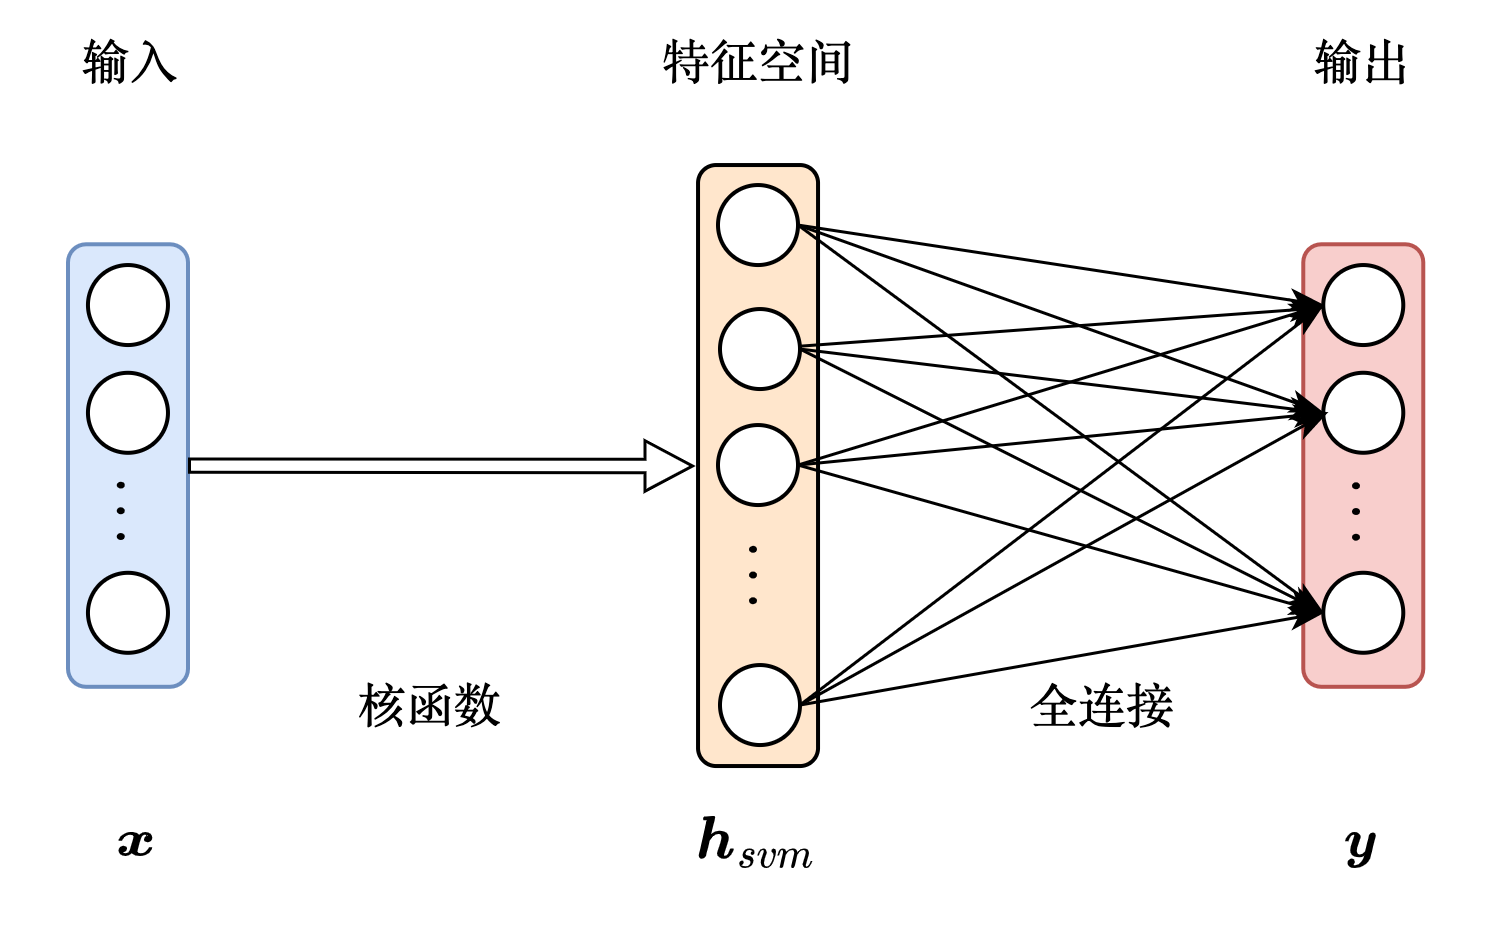
\includegraphics[width=\textwidth]{float/ch.intro/svm.png}
            \caption*{支持向量机(SVM)结构示例\label{fig:ch.intro.svm}}
        \end{minipage}
        \hfill
        \begin{minipage}[b]{0.45\textwidth}
            \centering
            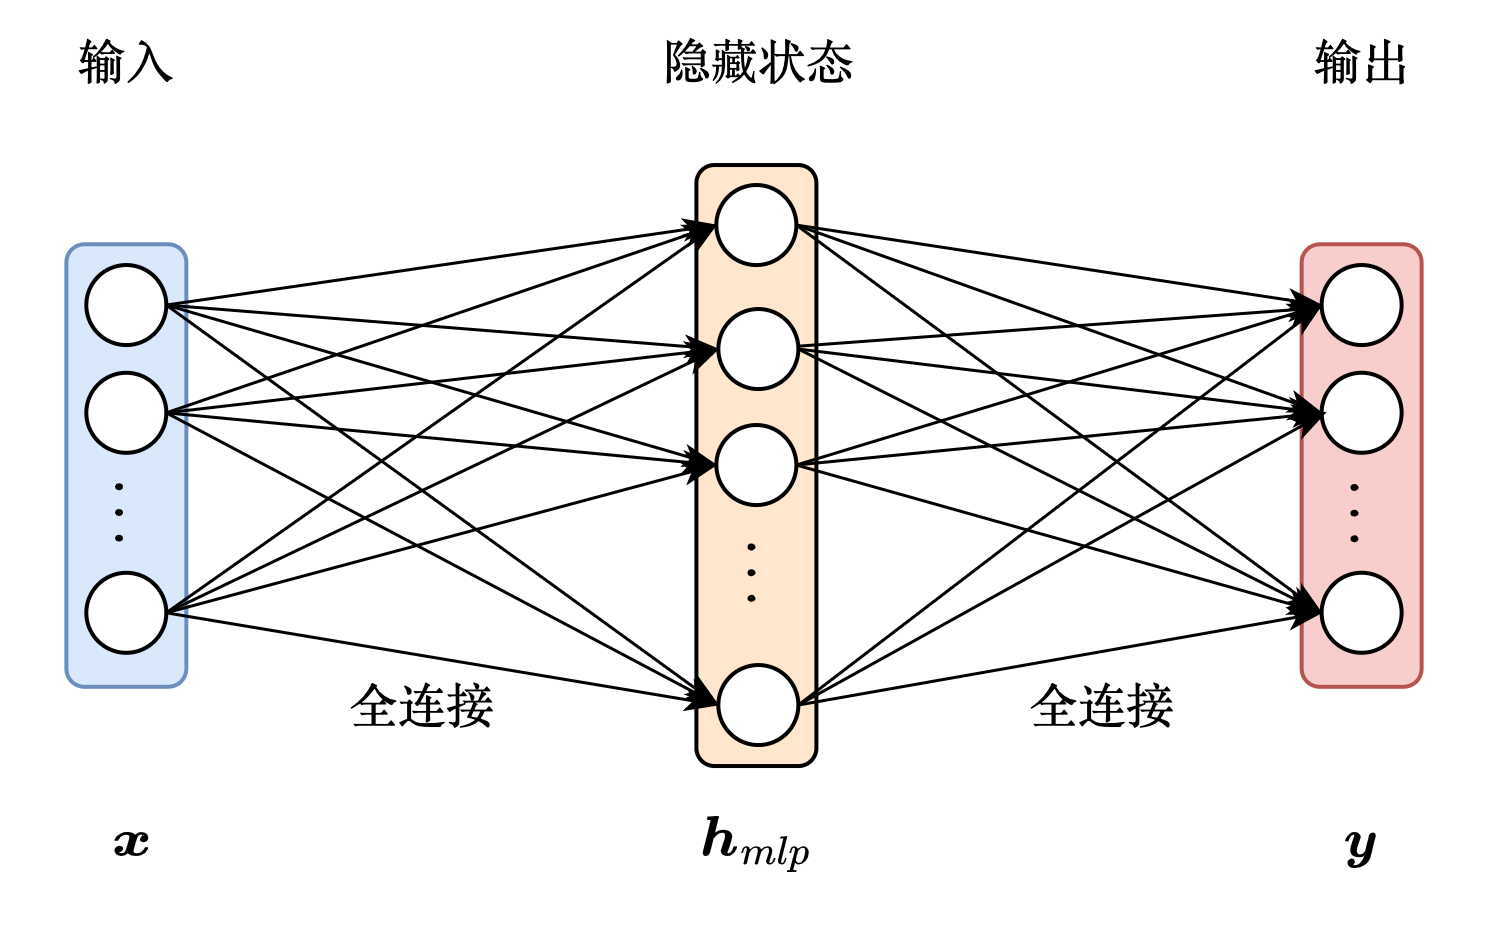
\includegraphics[width=\textwidth]{float/ch.intro/mlp.png}
            \caption*{多层感知机(MLP)结构示例\label{fig:ch.intro.mlp}}
        \end{minipage}
    \end{figure}

    以一组给定包含\(N\)个样本的时间序列数据集\(\mathbb{D} = \left\{\left(\x_{n}, \y_{n}\right) \in\left(\mathbb{R}^{T} \times \mathbb{R}^{H}\right)\right\}_{n=1}^{N}\)为例,对基于SVM与NN的预测建模技术与应用展开概述。

\end{frame}

\begin{frame}
    \frametitle{梯度下降}
    常有学者将基于梯度下降方法的神经网络模型称为反向传播神经网络(Back propagation neural network,BPNN)模型。

    \begin{itemize}
        \item 梯度下降:梯度下降训练方法中各层权重参数的优化方法
        \item 反向传播:梯度下降训练方法中计算各层权重参数梯度时所使用的链式法则梯度传导过程
    \end{itemize}

    以MLP为例:
    \begin{align*}
        \ell(\w) &= \frac{1}{N \times H} \sum^N_{n=1} \|\e_{n}\| ,\label{eq:ch.intro.mse}\\
        \e_{n} & = \y_n - f(\x_n).
    \end{align*}
    \centering
    \(\ell(\w)\)为神经网络预测模型在训练集\(\mathd\)上的MSE损失

\end{frame}

\begin{frame}
    \frametitle{梯度下降}

    核心思想:
    \begin{itemize}
        \item 基于神经网络模型中激活函数的连续性与可微性
        \item 向\(\w\)添加一个很小的动量\(\Delta_{\w}\),即\(\norm{\Delta_{\w}}\)很小,亦等价于\(\w + \Delta_{\w}\)近似\(\w\)
        \item 利用泰勒近似将复杂非凸的\(\ell(\w)\)函数优化问题当作一个简单的函数极小值问题
    \end{itemize}
    \begin{equation*}
        \ell({\w + \Delta_{\w}} ) \approx \ell({\w}) + \nabla_{\w}^{\mathrm{T}}\Delta_{\w}.
    \end{equation*}
    \(\nabla_{\w}\)表示\(\w\)在误差函数\(\w\)中的梯度。在最陡下降中,定义学习速率(Learning rate)为\(\eta \),且\(\eta  > 0\),因此:
    \begin{equation*}
        \Delta_{\w} = -\eta \nabla_{\w}. \label{eq:ch.intro.gd2}
    \end{equation*}
    当\(\eta \)足够小,可证:
    \begin{equation*}
        \ell({\w -\eta \nabla_{\w}} ) \approx \ell({\w})  -\eta  \nabla_{\w}^\trans \nabla_{\w} < \ell({\w}). \label{eq:ch.intro.lr}
    \end{equation*}
\end{frame}

\begin{frame}
    \frametitle{梯度下降的范式}

    \begin{algorithm}[H]
        \caption{神经网络模型梯度下降方法训练过程}
        % \renewcommand{\algorithmcfname}{算法}
        % \renewcommand{\algorithmicrequire}{\textbf{输入:}}
        % \renewcommand{\algorithmicensure}{\textbf{输出:}}
        \label{alg:ch.intro.gd}
        \begin{algorithmic}[1]
            \WHILE{未满足\(\vartheta\)界定的收敛条件}
            \STATE \(i\leftarrow i+1\)
            \STATE 基于\(\theta^i\),确定模型\(f \leftarrow  f \in \{\vartheta, \theta^i\}\)
            \STATE 基于数据集\(\mathd\)和模型\(f\),完成前馈过程\(f(\x)\),计算模型损失函数值\(\ell({\w}) \)
            \FOR{\(\w\) in \(\theta^i\) }
            \STATE 选取计算梯度所需的样本
            \STATE 根据反向传播链式法则计算梯度信息\(\nabla_{\w}\)
            \STATE 根据梯度下降更新公式更新权重参数\(\w\)
            \ENDFOR
            \ENDWHILE
            \RETURN {
                已完成更新过程的权重参数集合\(\theta \leftarrow \theta^i\)
            }
        \end{algorithmic}
    \end{algorithm}

\end{frame}

\begin{frame}
    \frametitle{深度学习建模方法}
    深度学习建模技术是机器学习建模技术中一类基于深度神经网络的建模方法。
    \begin{itemize}
        \item 海量数据的积累:CIFAR10,CIFAR100,ImageNet,WMT
        \item 计算能力的提升:GPU加速,分布式计算,并行计算
        \item 梯度下降的改进:SGD,Moment,Adam
        \item 通用框架的提出:TensorFlow,Pytorch
    \end{itemize}

    \begin{figure}
        \begin{minipage}[t]{0.55\textwidth}
            \begin{itemize}
                \item {
                    传统机器学习:人工经验建立特定的特征提取方法\begin{itemize}
                        \item 基于图像像素数值高斯分布描述图像特征的Fisher Vector方法
                        \item 基于语言文档内词频信息描述语句特征的词频-逆文档(TF-IDF)方法
                    \end{itemize}
                }
            \end{itemize}
        \end{minipage}
        \hfill
        \begin{minipage}[t]{0.44\textwidth}
            \begin{itemize}
                \item {
                    深度学习:依靠神经网络结构学习数据的抽象特征表示\begin{itemize}
                        \item CNN中的卷积结构
                        \item RNN中的循环结构
                    \end{itemize}
                }
            \end{itemize}
        \end{minipage}
    \end{figure}
\end{frame}

\begin{frame}
    \frametitle{深度学习示例}

    \begin{figure}[t!]
        \centering
        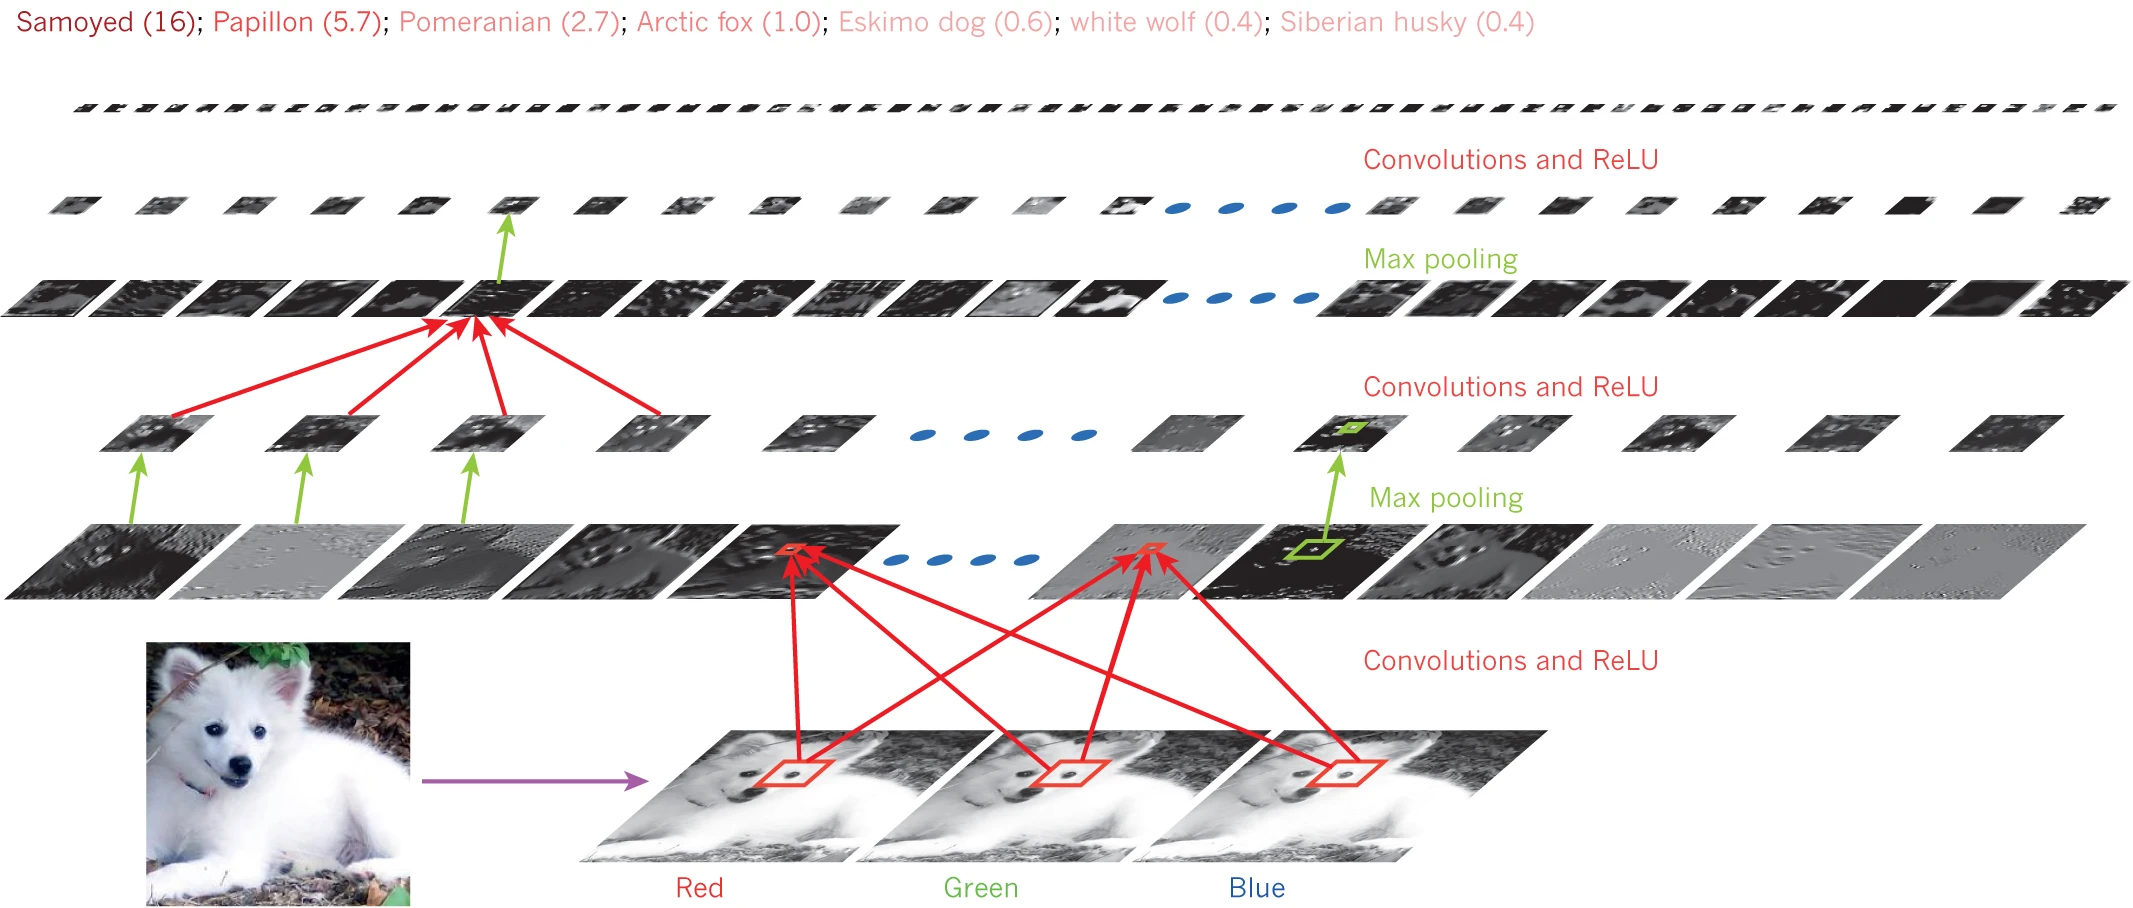
\includegraphics[width = \linewidth]{float/ch.intro/lecun.png}
        \caption*{卷积神经网络图像分类模型示例(引用于Lecun et al. “Deep Learning.” Nature, 2015, 521.7553: 436-444)}
    \end{figure}

\end{frame}

\begin{frame}
    \frametitle{模型选择问题}

    对于由超参数\(\vartheta\)和权重参数\(\theta\)所定义的深度学习预测模型\(f\),其模型选择问题便是如何选择合适的\(\vartheta\)与\(\theta\)从而提升模型\(f\)预测性能的问题。

    \begin{itemize}
        \item 权重参数\(\theta\)的优化研究 \(\rightarrow\) 梯度下降方法的改进
        \item 超参数\(\vartheta\)的优化研究 \(\rightarrow\) 神经网络结构的优化
    \end{itemize}

    \vspace{0.5em}
    神经网络结构的分解:
    \begin{itemize}
        \item 表征结构
        \begin{itemize}
            \item 隐藏结构 \(\rightarrow\) 神经网络结构搜索 (NAS)
                \begin{itemize}
                    \item 启发式优化、强化学习 \(\rightarrow\) 计算开销大,选择耗时长
                \end{itemize}
            \item 输入结构 \(\rightarrow\) 预测领域的多输入特征选择
            \begin{itemize}
                \item 封装法更优 \(\rightarrow\) 多时步维度的输入特征结构
            \end{itemize}
        \end{itemize}
        \item 输出结构 \(\rightarrow\) 预测领域的多输出策略优化
 \begin{itemize}
            \item MIMO策略,Direct策略,Iterative策略
            \begin{itemize}
                \item MIMO更优 \(\rightarrow\) MIMO策略下依然存在多种输出结构
            \end{itemize}
        \end{itemize}
    \end{itemize}

\end{frame}

\begin{frame}
    \frametitle{模型选择研究}

    \(\theta\)依赖于超参数\(\vartheta\):
    \begin{itemize}
        \item 模型神经网络结构参数(如CNN模型中卷积层层数、卷积核宽度和卷积核数量等等)
        \item 梯度下降方法参数(如SGD方法中的学习速率、批次样本选取数量和动量惯性系数等等)
    \end{itemize}

    \begin{center}
        不同的\(\vartheta\)必然会导致\(\theta\)的差异
    \end{center}

\end{frame}

\begin{frame}
    \frametitle{模型选择过程}
\begin{algorithm}[H]
    \caption{基于梯度下降方法的神经网络预测建模技术模型选择过程}
    \begin{algorithmic}[1]

        \WHILE{未满足模型选择方法界定的收敛条件}
        \STATE \(j\leftarrow j+1\)
        \STATE 从超参数集合\(\vartheta\)的搜索空间\(\Omega\)中选择或更新出当前的超参数集合\(\vartheta^j\)
        \STATE 基于\(\vartheta^j\):\\
        \hspace{2em}执行梯度下降算法所示步骤\\
        \hspace{2em}得到当前\(\vartheta^j\)试验下的权重参数集合\(\theta|\vartheta^j\)\\
        \hspace{2em}确定模型\(f \leftarrow  f \in \{\vartheta^j, \theta|\vartheta^j\}\)
        \STATE 基于数据集\(\mathd\)和模型\(f\),计算模型误差
        \STATE 基于模型误差与超参数更新方法:\\
        \hspace{2em}更新最优的神经网络超参数集合\(\vartheta^*\)\\
        \hspace{2em}更新最优的神经网络超参数集合\(\theta^* \leftarrow  \theta|\vartheta^*\)
        \ENDWHILE
        \RETURN {
            已完成更新过程的超参数集合\(\vartheta \leftarrow \vartheta^*\)与权重参数集合\(\theta \leftarrow \theta^*\)
        }
    \end{algorithmic}
\end{algorithm}   

\end{frame}

\begin{frame}{模型选择挑战}
    \begin{figure}
        \begin{minipage}[b]{0.45\textwidth}
            深度学习预测建模技术所面临的模型选择挑战尤为突出。
            \vspace{2em}
            \begin{itemize}
                \item 更多的权重参数以及更加复杂的梯度计算方式,导致模型选择效率低
                \item 复杂的神经网络结构加深了超参数搜索空间的复杂程度,导致模型选择效果弱
            \end{itemize}
        \end{minipage}
        \quad
    \begin{minipage}[b]{0.45\textwidth}
        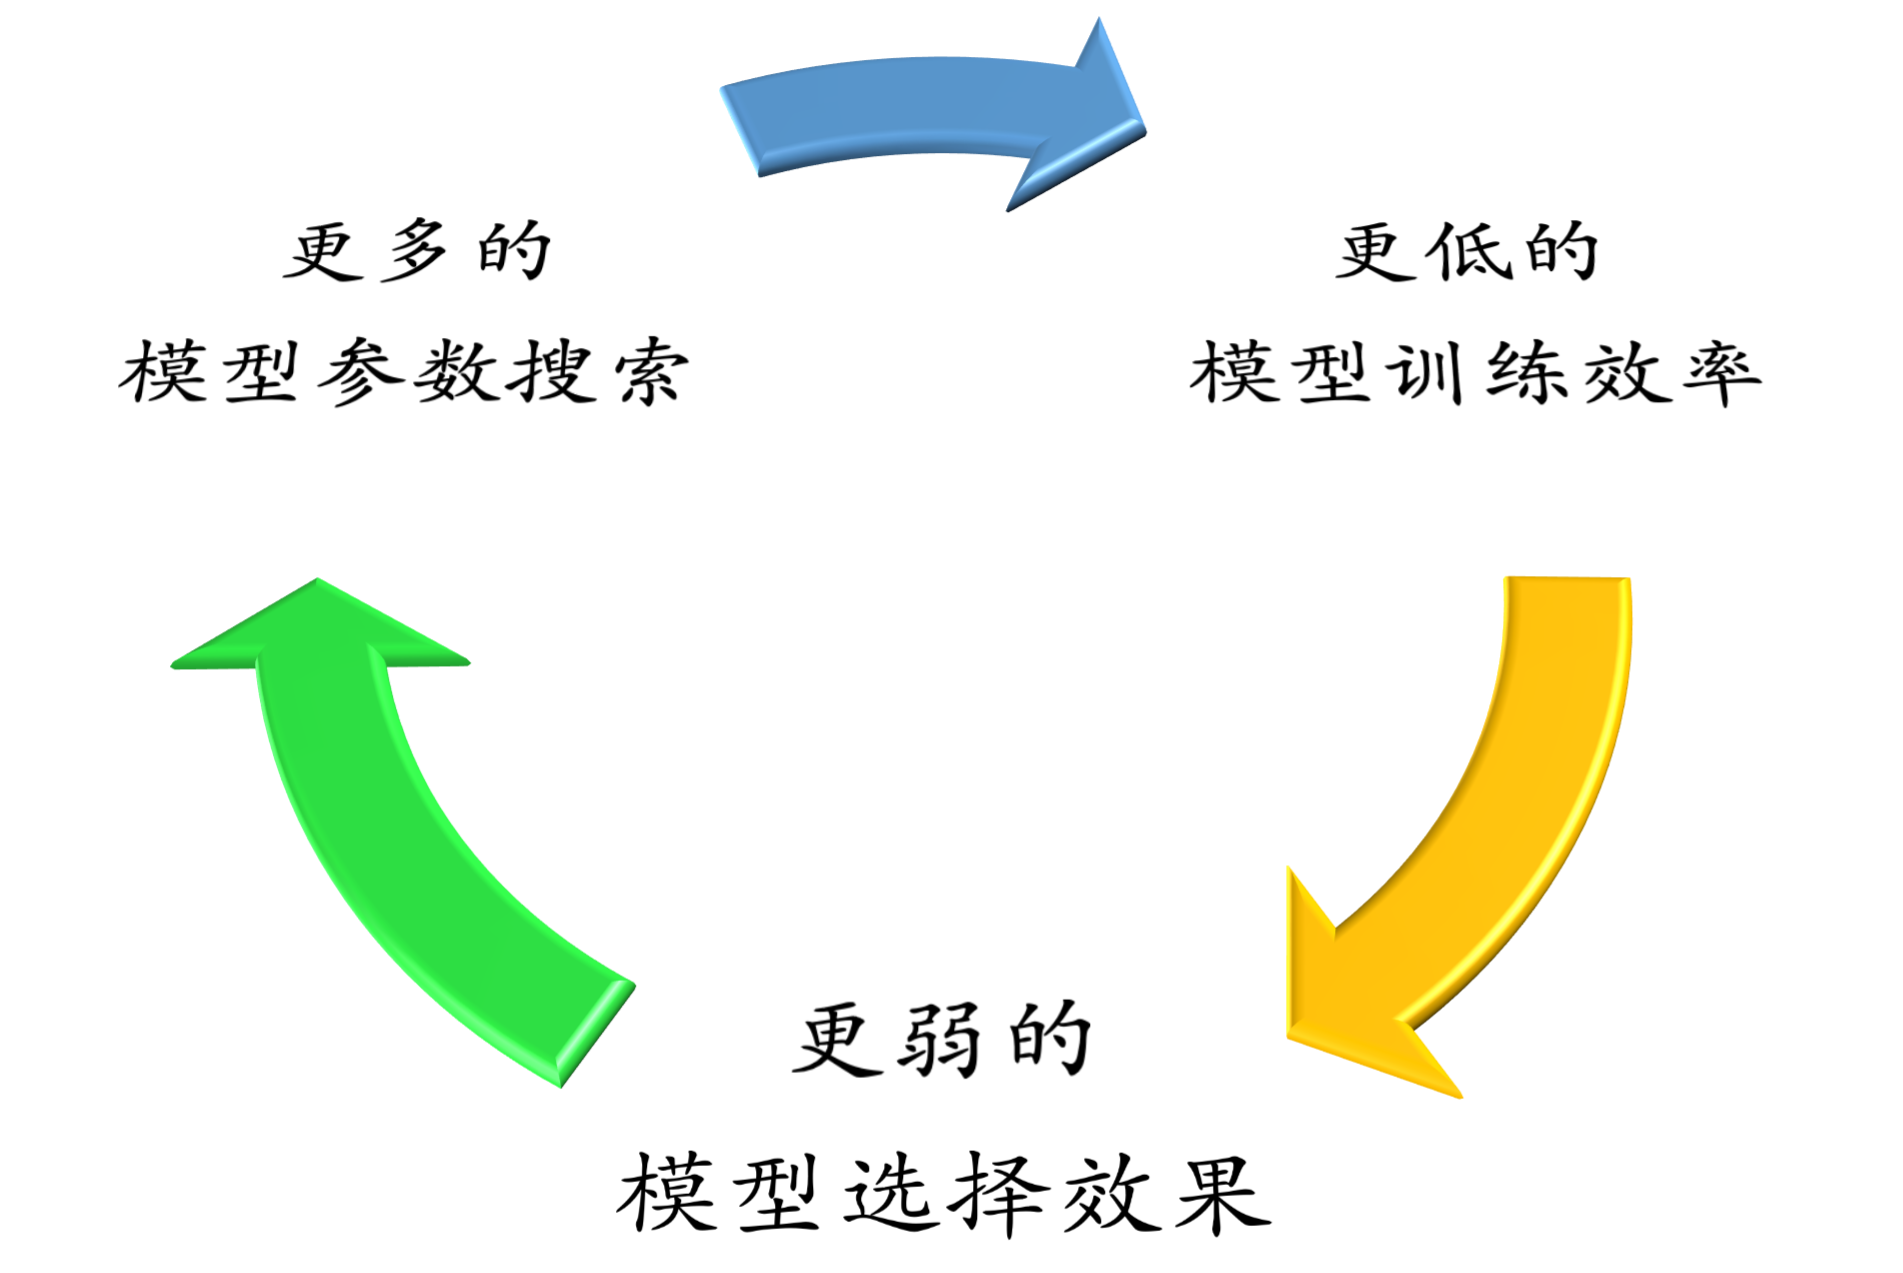
\includegraphics[width=\textwidth]{float/ch.intro/circle.png}
    \end{minipage}
    \end{figure}
    \end{frame}

    \begin{frame}
        \frametitle{随机映射方法研究概况}
        随机映射是一种采用非迭代学习机制的MLP建模方法。
    
        \begin{figure}[H]
            \begin{subfigure}[b]{0.25\textwidth}
                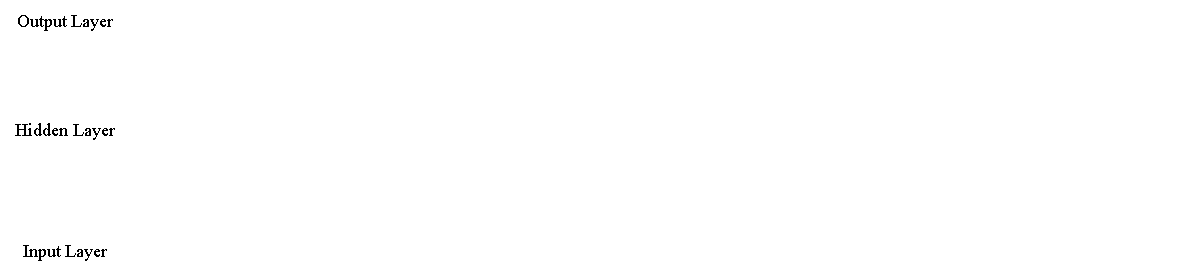
\includegraphics[height=\linewidth]{float/ch.cnn/layer.pdf}
                \caption*{}
            \end{subfigure}
            \hspace*{-0.15\textwidth}
            \begin{subfigure}[b]{0.25\textwidth}
                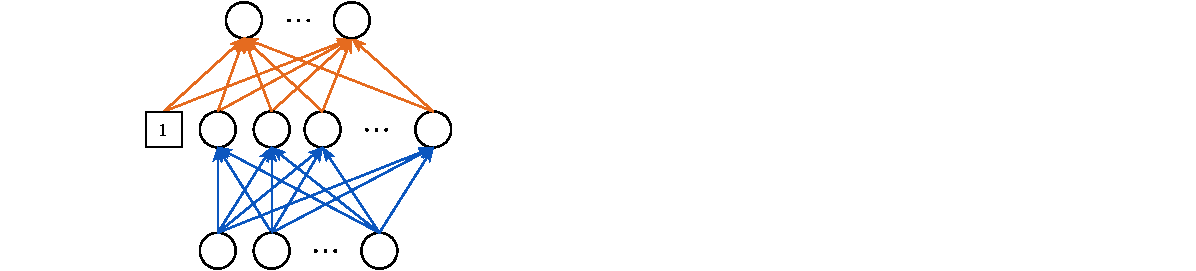
\includegraphics[height=\linewidth]{float/ch.cnn/schmidt.pdf}
                \caption{Schimidt网络}
            \end{subfigure}
            \hspace*{0.03\textwidth}
            \begin{subfigure}[b]{0.25\textwidth}
                
\includegraphics[height=\linewidth]{float/ch.cnn/rvfl.pdf}
                \caption{RVFL网络}
            \end{subfigure}
            \hspace*{\fill}
            \begin{subfigure}[b]{0.25\textwidth}
                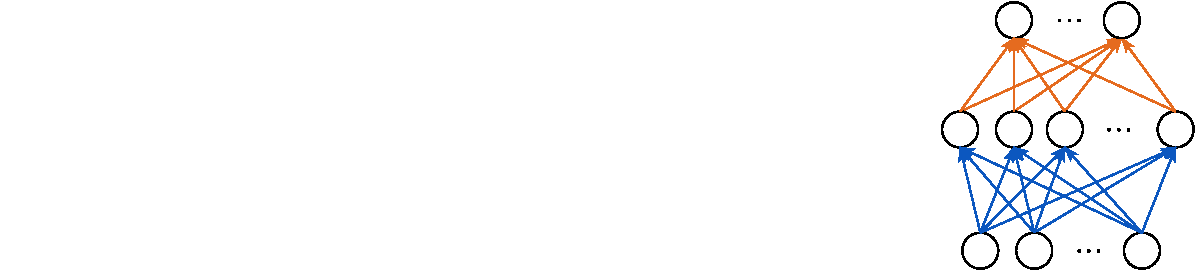
\includegraphics[height=\linewidth]{float/ch.cnn/elm.pdf}
                \caption{ELM网络}
            \end{subfigure}
            \caption*{\label{fig:randomnet}蓝色线表示固定的随机初始化权重,黄色线表示闭式求解得输出权重。}
        \end{figure}
        
    \end{frame}

    \begin{frame}
        \frametitle{随机映射建模过程}
    
        以MLP为例:随机映射多层感知机(Stochastic multiple percentage, SMLP)模型的预测过程为:
        \begin{align*}
            f_{smlp}(\x) &= \w_{out}\h_{smlp}, \\
            \h_{smlp} &= \sigma (\w_{hid}\x). \notag
        \end{align*}
        其模型损失函数依然保持MSE损失形式
        \begin{align*}
            \w_{out} &= \argmin_{\w_{out}} \norm{\y - \w_{out}\h_{smlp}} \\ 
            & = \y \h_{smlp}^{\trans} (\h_{smlp}\h_{smlp}^\trans)^{-1}. \notag
        \end{align*}
    
        支持向量机模型是一种SMLP模型的特例
    \end{frame}

    \begin{frame}
        \frametitle{SMLP的收敛性质}
    
        传统的SMLP模型避免了梯度下降训练计算开销高的问题,但这种权重随机机制使其模型性能的收敛性与稳定性受到质疑。
    
        针对于此:
        \begin{itemize}
            \item Huang等\footnote{Huang et al. "Universal approximation using incremental constructive feedforward networks with random hidden nodes." IEEE Trans. Neural Networks 17.4 (2006): 879-892.}基于递归添加神经元的方式构造了一种增长极限感知机(Incremental extreme learning machine,IELM),并证明了IELM对于任意连续有界目标函数的学习收敛能力。
            \item Wang等\footnote{Wang et al. "Stochastic configuration networks: Fundamentals and algorithms." IEEE transactions on cybernetics 47.10 (2017): 3466-3479.}通过迭代增加隐藏层神经元,基于监督机制闭式挑选神经元隐藏层权重,全局更新输出层权重的方式,构造出增长的SMLP模型,并证明了SCN的普适逼近性质(Universal approximation property)。
        \end{itemize}
        
    \end{frame}

    \begin{frame}
        \frametitle{随机映射深度学习建模技术}
    
        随机映射RNN的研究:
        \begin{itemize}
            \item Jaeger等\footnote{Jaeger et al. "Harnessing nonlinearity: Predicting chaotic systems and saving energy in wireless communication." science 304.5667 (2004): 78-80.}在2001年提出随机映射RNN,称其为状态回声网络(Echo state network,ESN)。
            \item 技术:Leaky ESN,Growing ESN,Deep ESN,Regularize ESN
            \item 应用:电力负荷预测,原油价格预测
        \end{itemize}
    
        随机映射CNN的研究:
        \begin{itemize}
            \item He等\footnote{He et al. "A powerful generative model using random weights for the deep image representation." Advances in Neural Information Processing Systems 29 (2016).}发现随机映射CNN在纹理生成和风格迁移等任务上具有不亚于梯度下降训练CNN的表现。
            \item 预测研究较少
        \end{itemize} 
    \end{frame}

    \begin{frame}
        \frametitle{随机映射深度学习预测建模技术}
    
        由此,针对时间序列深度学习预测技术模型选择挑战中的低效问题,构造基于随机映射的深度学习预测建模技术是一种有效的解决途径
        \begin{itemize}
            \item 深度学习建模技术优异的预测潜能
            \item 随机映射建模技术高效的建模效率
        \end{itemize}
    
        \vspace{1em}
        随机映射深度学习预测建模技术的挑战:
        \begin{itemize}
            \item 建模效率的提高建立在预测性能的牺牲上
            \item 更高的模型选择要求
        \end{itemize}
    
    \end{frame}


\begin{frame}
    \frametitle{技术研究体系}
\vspace{-0.5em}
\centering
\begin{figure}[!th]
    \centering
    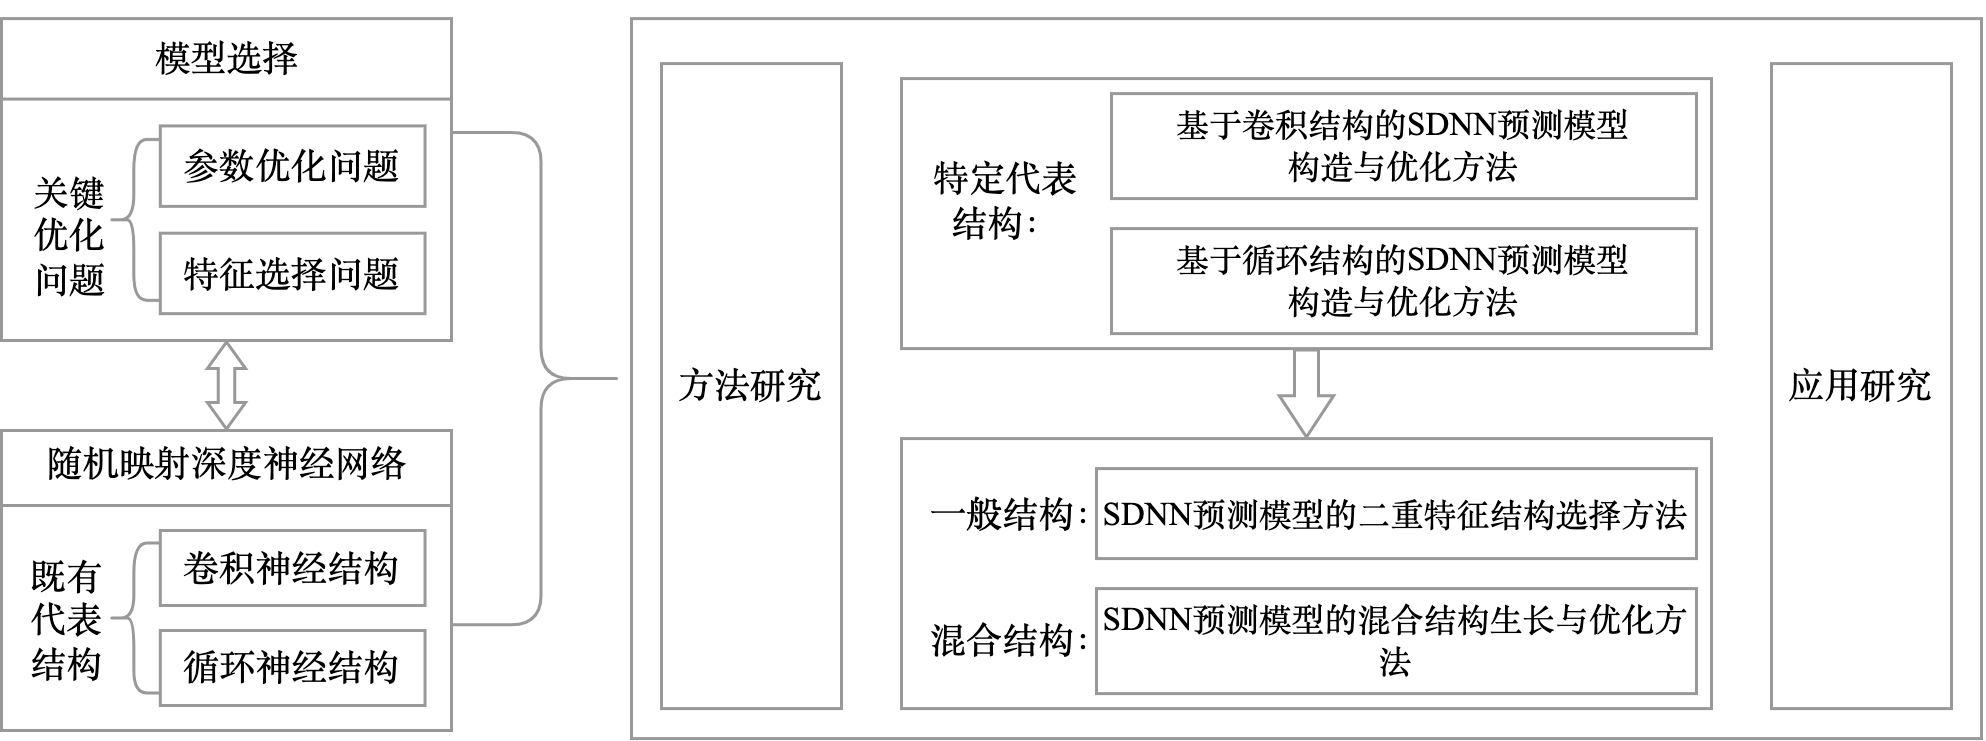
\includegraphics[width=0.88\linewidth]{float/ch.intro/thesis.png}
    
\end{figure}
\end{frame}

\begin{frame}
    \frametitle{研究意义}

    \textbullet ~~~ 在理论层面,本论文将深入研究不同神经网络结构下的SDNN预测模型和新的理论分析框架,如构建基于卷积结构和混合结构的SDNN预测模型的预测误差收敛性分析框架,直观理解SDNN预测模型的构造与决策逻辑

    \textbullet ~~~在方法层面,本论文将构造多套预测模型构造与优化方法,包括适用于卷积结构、循环结构、一般结构至混合结构SDNN模型的优化技术,形成从特定到一般再到混合的综合技术体系与框架,为SDNN预测建模技术的复杂模型选择问题提供新颖的方法与思路

    \textbullet ~~~在现实层面,本论文将立足于现实时间序列预测任务的多个场景,包括公共卫生领域中的流感阳性样本率预测任务、能源市场中的原油价格预测任务、金融市场中的股票指数预测任务、大气污染中的PM2.5预测任务、电力系统中的电力负荷与电力价格预测任务等
    
\end{frame}
\section{cnn}
\begin{frame}{Conv-SDNN预测模型——引言}
    基于卷积结构的SDNN预测模型:随机映射CNN模型
    \begin{itemize}
        \item 随机映射CNN在图像生成任务(纹理生成、风格迁移)上具有不亚于梯度下降训练CNN的表现
    \end{itemize}
    \vspace*{-0.5em}
    \begin{figure}
        \centering
        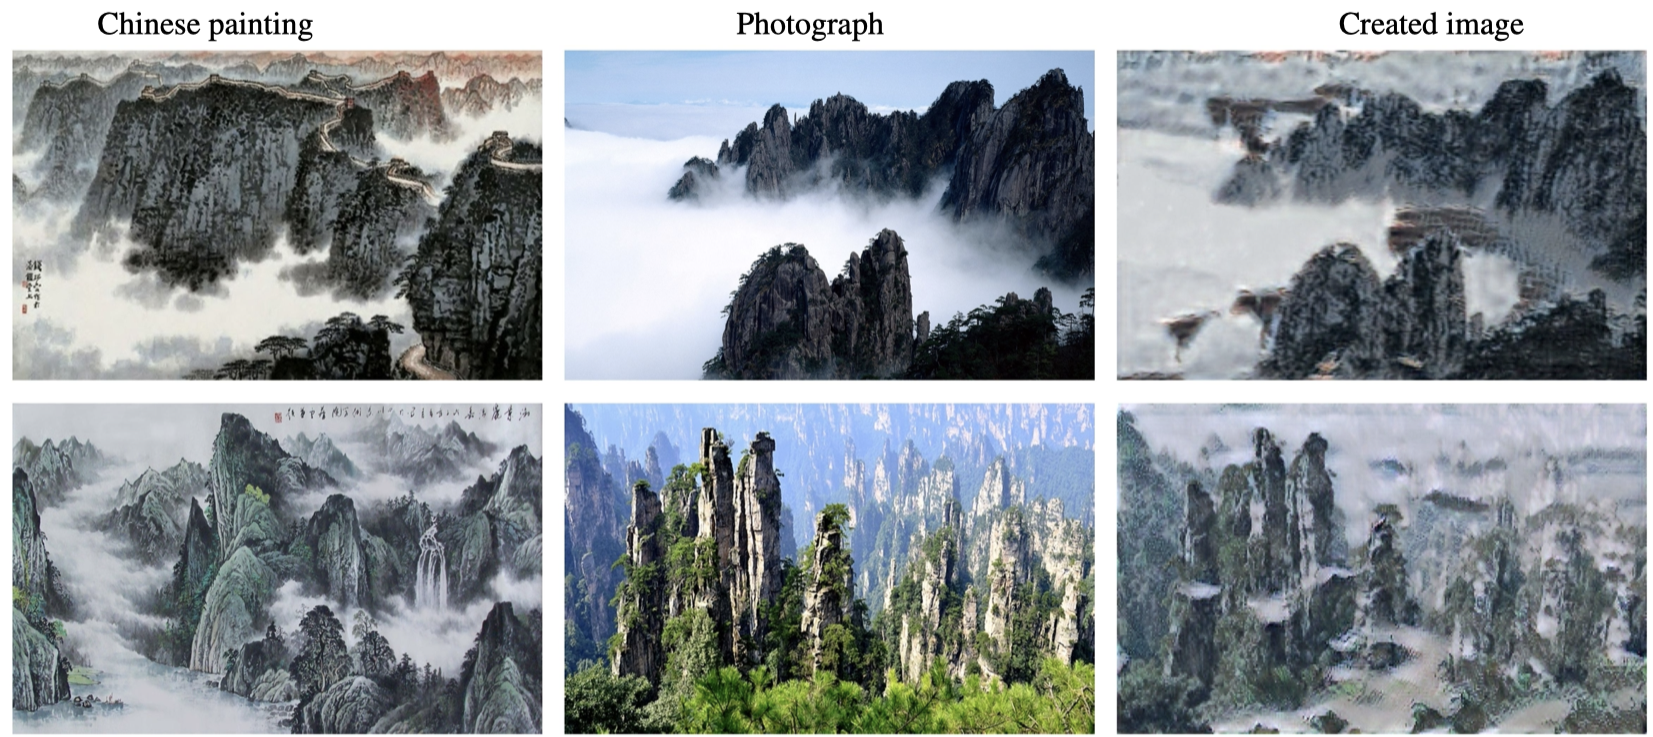
\includegraphics[width=0.9\linewidth]{float/ch.cnn/ranVGG.png}
    \end{figure}
\end{frame}

\begin{frame}{Conv-SDNN预测模型——引言}
    随机映射CNN模型研究:
    \begin{itemize}
        \item 一维随机映射CNN在一些人工时间序列预测数据集上展现出比MLP模型更好的拟合性能(Yu et al. 2019)
    \end{itemize}
    \vspace*{-0.5em}
    \begin{figure}
        \centering
        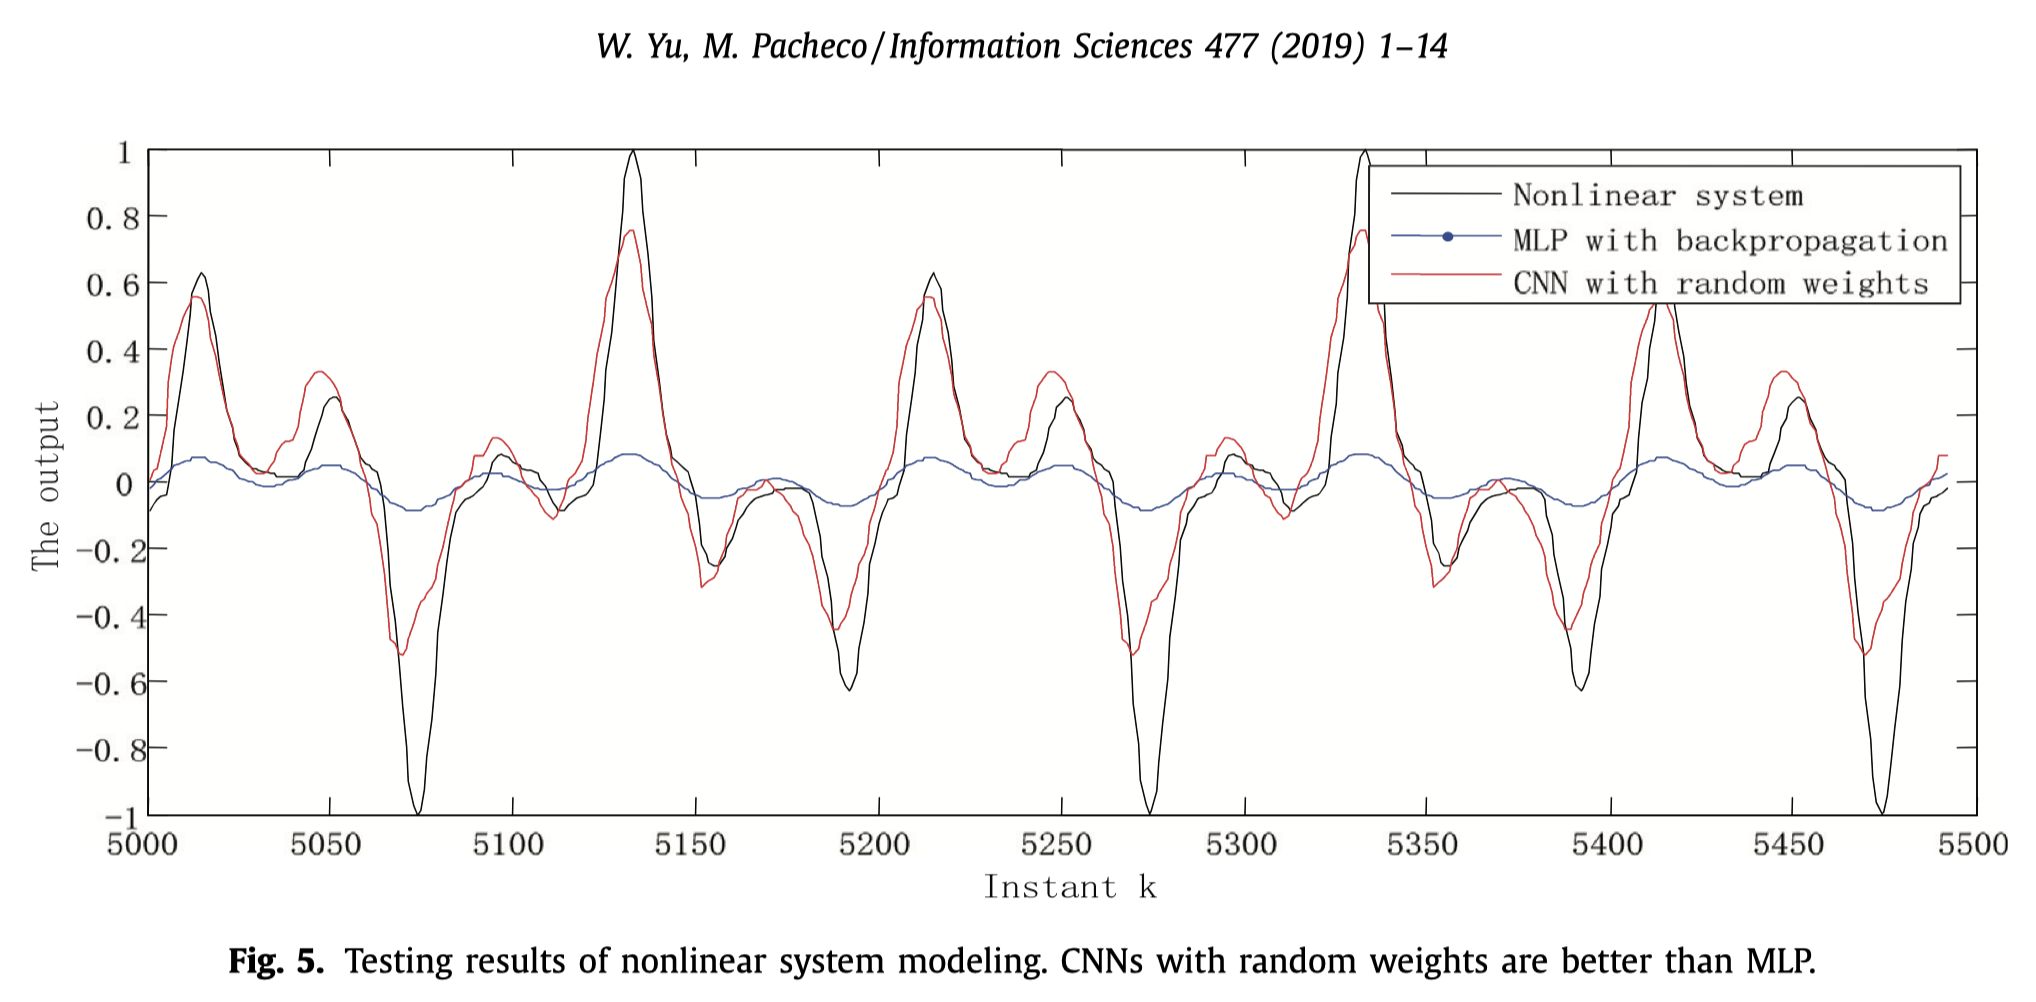
\includegraphics[width=0.9\linewidth]{float/ch.cnn/yu.png}
    \end{figure}
\end{frame}

\begin{frame}{Conv-SDNN预测模型——引言}
    随机映射CNN模型研究归纳:
    \begin{itemize}
        \item 既有研究较少,已有随机映射CNN模型性能有限,亟待新的随机映射CNN预测模型及其构造技术
    \end{itemize}

    \vspace*{0.5em}
    本章贡献:
    \begin{itemize}
        \item 基于误差反馈随机映射的随机映射CNN预测模型构造方法
              \begin{itemize}
                  \item 通过递归生成随机映射卷积核的方式提高了模型构造效率
                  \item 借助基于误差反馈策略保证了所构造模型的理论收敛性
              \end{itemize}
        \item 引入贪心算法解决模型构造中随机映射卷积核的选择问题
              \begin{itemize}
                  \item 自适应的在单卷积层内具备不同卷积宽度的卷积核
              \end{itemize}
        \item 与梯度下降深度学习模型和传统随机映射模型相比,ESM-CNN具有优秀的预测性能与建模效率
    \end{itemize}

\end{frame}


\begin{frame}{Conv-SDNN预测模型——CNN预测模型}


    \begin{figure}[!t]
        % \newlength{\twosubht}
        % \newsavebox{\twosubbox}
        \centering
        % \begin{minipage}{0.8\textwidth}
        %     \includegraphics[width = \textwidth]{float/ch.eto/esc.png}
        %     \caption*{回声状态卷积(ESC)结构}
        % \end{minipage}
        \begin{minipage}{0.8\textwidth}
            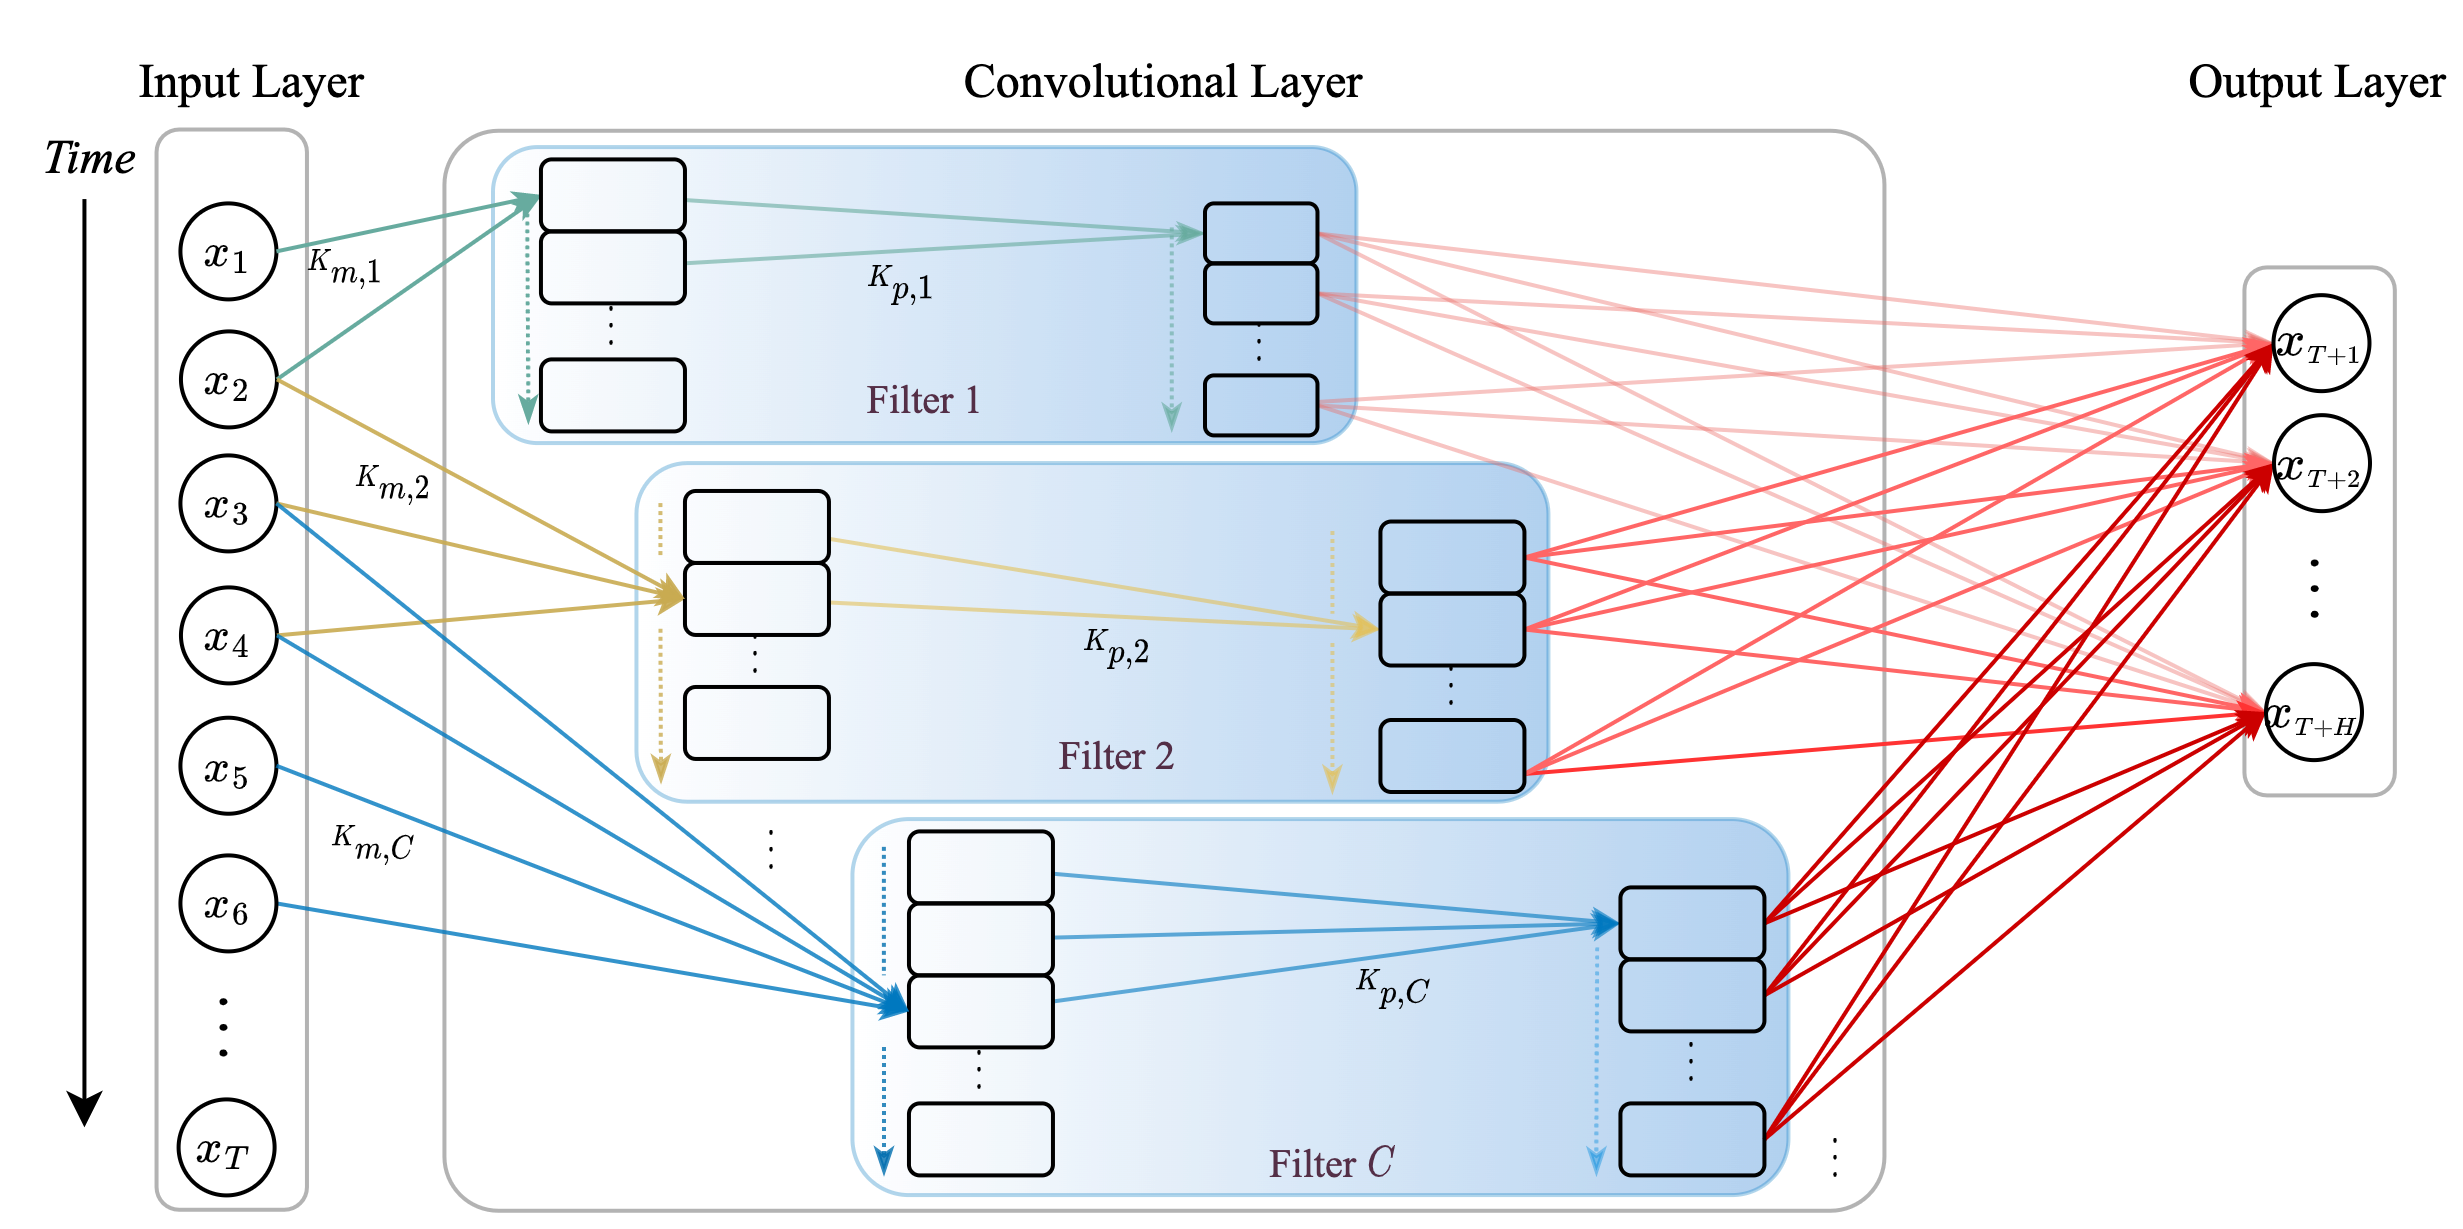
\includegraphics[width = \textwidth]{float/ch.cnn/esm-cnn.png}
            \caption*{CNN结构}
        \end{minipage}    
        % \caption{\label{fig:archMix} 基于循环神经网络与卷积神经网络的混合神经网络结构示例.}
    \end{figure}



\end{frame}

\begin{frame}
    \frametitle{Conv-SDNN预测模型——误差反馈随机映射构造方法}
    \begin{itemize}
        \item 过在单卷积层内递归增长添加固定随机初始化权重卷积核的方式构造CNN隐藏结构
        \item 利用误差反馈闭式计算新增卷积核所对应的输出权重参数
    \end{itemize}

    对于一个已具有$C$个卷积核的单卷积层ESM-CNN
    \begin{equation*}
        f_C= \sum^C_{j=1}\sum^{T-K+2}_{i=0} \beta_j^i p_j^i
    \end{equation*}

    当前预测误差为:
    \begin{equation*}
        e_C = y - f_C = [e_C^1,\ldots, e_C^H].
    \end{equation*}

    新增卷积核所对应的全连接输出层权重将基于当前模型的预测误差$e_C$反馈,通过OLM加以求解:

    \vspace{-1.5em}
    \begin{equation*}
        \left[\beta_{{C+1}}^0, \ldots, \beta_{{C+1}}^{T-K+2} \right]=\argmin _{\beta}\|e_C -\sum_{i=0}^{T-K+2} \beta_{C+1}^i p_{C+1}^i \|.
    \end{equation*}
\end{frame}

\begin{frame}
    \frametitle{Conv-SDNN预测模型——拟合收敛性}

    定义ESM-CNN的预测误差中间项为:$\tilde{e}_{C+1}^{\, 0}, \ldots, \tilde{e}_{C+1}^{\, T-K+2} $,新增卷积核所对应的全连接输出层权重中间项为:$\tilde{\beta}_{C+1}^{\, 0}, \ldots, \tilde{\beta}_{C+1}^{\, T-K+2}$,中间项之间的计算关系为:
    \begin{alignat*}{2}
         & \tilde{e}_{C+1}^{\, i+1}       & = & \mspace{18mu} \tilde{e}_{C+1}^{\, i}-\tilde{\beta}_{C+1}^{\, i+1} p_{C+1}^{i+1}, \quad i = 0,\ldots,T-K+1,                                        \\
        \shortintertext{其中,}
         & \tilde{\beta}_{C+1}^{\, i+1}   & = & \mspace{18mu} [\tilde{\beta}_{C+1}^{\, i+1,1}, \ldots,\tilde{\beta}_{C+1}^{\, i+1,h},\ldots, \tilde{\beta}_{C+1}^{\, i+1,H}],                     \\
         & \tilde{\beta}_{C+1}^{\, i+1,h} & = & \mspace{18mu} \left\langle \tilde{e}_{C+1}^{\, i,h}, p_{C+1}^{\, i+1}\right\rangle /\left\|p_{C+1}^{\, i+1}\right\|^{2} , \quad h= 1, \ldots, H .
    \end{alignat*}
    可证:
    \vspace{-1em}
    \begin{align*}
            & \|\tilde{e}_{C+1}^{\, i+1}\|^2-\|\tilde{e}_{C+1}^{\, i}\|^2 \\
        ={} & \sum_{h=1}^{H}
        \left(
        \langle \tilde{e}_{C+1}^{\, i,h}-\tilde{\beta}_{C+1}^{\, i+1,h} p_{C+1}^{i+1}
        ,
        \tilde{e}_{C+1}^{\, i,h}-\tilde{\beta}_{C+1}^{\, i+1,h} p_{C+1}^{i+1} \rangle
        -
        \langle \tilde{e}_{C+1}^{\, i,h}, \tilde{e}_{C+1}^{\, i,h} \rangle
        \right)                                                           \\
        ={} & \sum_{h=1}^{H}
        \left(
        - {\langle \tilde{e}_{C+1}^{\, i,h}, p_{C+1}^{\, i+1} \rangle}^2 / \left\|p_{C+1}^{\, i+1}\right\|^{2}
        \right)      \leq 0
    \end{align*}
\end{frame}

\begin{frame}
    \frametitle{Conv-SDNN预测模型——拟合收敛性}

    该性质在$\left\|\tilde{e}_{C+1}^{\, 0}\right\|^{2}$与$\left\|e_{C}\right\|^{2}$间仍然保持,
    因此,ESM-CNN的预测误差收敛性如下:
    $$
        \|e_{C+1}\|^2  \; \leq \|\tilde{e}_{C+1}^{\, T-K+2}\|^2 \; \leq \|\tilde{e}_{C+1}^{\,0}\|^2 \; \leq \|{e}_{C}\|^2 .
    $$

    方法优势:
    \begin{itemize}
        \item 迭代局部更新输出层权重的方式具有更小的计算开销,这种低开销优势会随隐藏层结构的增大同时扩大
        \item 随着卷积层中递归新增卷积核的不断加入,链接至输出层的池化特征图向量维度会同时倍数增大,与预测目标维度相比过大的特征维度会导致闭式求解算法的病态问题(Ill-posed problem)
        \item 基于误差反馈递归更新输出权重构造的预测模型能在神经网络隐藏构造的过程中不断弥补上步预测误差,同时,这种历史输出权重保持固定的方式在一定程度上承担了正则化的作用,从而增强了所构造模型的性能稳定性
    \end{itemize}
\end{frame}

\begin{frame}
    \frametitle{Conv-SDNN预测模型——卷积核选择方法}

    针对ESM-CNN预测模型构造中的卷积核选择问题,本章节提出了一种基于贪心算法的卷积核选择方法,使得ESM-CNN具有在单卷积层中同时具备不同宽度的卷积核结构,以此增强模型对于不同尺度时间序列特征的学习建模能力。

    本节提出了一种卷积核评分$\Delta_{{C+1, s}}$,计算如下:
    \begin{align*}
        \Delta_{{C+1},s} & = \| e_{C+1,s} \|^2 - \| e_{C} \|^2 \notag                                                                        \\
        {}               & = \|\ e_C -\sum_{i=0}^{T-K^{\prime}+2} \beta_{C+1, s}^i p_{C+1, s}^i \|^2 -  \| e_{C} \|^2 \label{eq:filterScore}
    \end{align*}


    基于所提的卷积核评分,实现最好预测效果提升的备选卷积核$p_{C+1}^{*}$将被选出作为新增卷积核正式加入当前神经网络结构,该过程可被表述为:
    \begin{equation*}\label{eq:scselection}
        p_{C+1}^{*} = \argmax\limits_{p_{{C+1},s}} \{ \Delta_{{C+1},s}, s = 1,\ldots,S \}.
    \end{equation*}

\end{frame}

\begin{frame}
    \frametitle{Conv-SDNN预测模型——实验设计}

    \begin{table}[!t]
    \centering
    \caption{数据集信息 \label{tab:app_data}}
    \begin{tabularx}{\textwidth}{lccccY}
    % \caption{数据集信息 \label{tab:app_data}}\\
    \toprule
    数据集名称      & 平稳性 & 趋势性 & 季节性 &  起始截止日期  & 数据集大小 \\ \midrule
    AR1          & \xmark      & 0.97      & 0.09        & -                           & 500         \\
    BTC          & \xmark      & 0.99      & 0.66        & 05/25/2020 $\sim$ 03/20/2021 & 2181        \\
    ILI          & \cmark      & 0.51      & 0.61        & 01/15/2010 $\sim$ 04/15/2020 & 535         \\
    BRENT-weekly & \xmark      & 0.97      & 0.07        & 05/15/1987 $\sim$ 04/30/2021 & 1773        \\
    BRENT-daily  & \xmark      & 0.97      & 0.06        & 05/20/1987 $\sim$ 05/03/2021 & 8620        \\
    WTI-weekly   & \xmark      & 0.96      & 0.08        & 01/03/1986 $\sim$ 04/30/2021 & 1844        \\
    WTI-daily    & \xmark      & 0.96      & 0.07        & 01/02/1986 $\sim$ 05/03/2021 & 8904        \\
    S\&P 500           & \xmark      & 0.99      & 0.40        & 12/31/2009 $\sim$ 11/15/2017 & 1984        \\
    NASDAQ       & \xmark      & 0.99      & 0.27        & 12/31/2009 $\sim$ 11/15/2017 & 1984        \\
    DJI          & \xmark      & 0.99      & 0.40        & 12/31/2009 $\sim$ 11/15/2017 & 1984        \\
    NYSE         & \xmark      & 0.98      & 0.45        & 12/31/2009 $\sim$ 11/15/2017 & 1984        \\ \bottomrule
    \end{tabularx}
    \end{table}

\end{frame}

\begin{frame}
    \frametitle{Conv-SDNN预测模型——实验设计}

    \begin{figure}
        \begin{minipage}[t]{0.5\textwidth}
            对比模型:
            \begin{itemize}
                \item 统计预测模型
                      \begin{itemize}
                          \item Naive、ARIMA、Holt’s Winters
                      \end{itemize}
                \item 随机映射模型
                      \begin{itemize}
                          \item RVFL、IELM、SCN
                      \end{itemize}
                \item 深度学习模型
                      \begin{itemize}
                          \item GS-CNN、DeepAR、CLSTM
                      \end{itemize}
                \item 消融实验模型
                      \begin{itemize}
                          \item 移除卷积核选择 \\ \(\rightarrow\) ES-CNN
                          \item 移除误差反馈与卷积核选择 \\ \(\rightarrow\) Stoc-CNN
                      \end{itemize}
            \end{itemize}
        \end{minipage}
        \hfill
        \begin{minipage}[t]{0.45\textwidth}
            评价指标:
            \begin{itemize}
                \item 百分比误差
                      \begin{itemize}
                          \item MAPE、SMAPE
                      \end{itemize}
                \item 绝对值误差
                      \begin{itemize}
                          \item RMSE
                      \end{itemize}
            \end{itemize}

            \begin{equation*}
                MAPE = \frac1N \sideset{}{_{i=1}^N} \sum \abs{\frac{y_{i} - \hat  y_{i}}{y_i}}.
            \end{equation*}
            \begin{equation*}
                SMAPE = \frac1N \sideset{}{_{i=1}^N} \sum \abs{\frac{y_{i} - \hat  y_{i}}{y_i + \hat  y_{i}}}.
            \end{equation*}
            \begin{equation*}
                RMSE = \sqrt{\frac1N \sideset{}{_{i=1}^N} \sum ({y_{i} - \hat  y_{i}})^2 }.
            \end{equation*}
        \end{minipage}
    \end{figure}
\end{frame}


\begin{frame}
    \frametitle{Conv-SDNN预测模型——实验步骤}

    \begin{itemize}
        \item 数据集预处理:基于Z-score方法\footnote{https://scikit-learn.org/stable/modules/preprocessing.html\#preprocessing-scaler.}归一化至标准正太分布
        \item 数据集切分:按照0.64,0.16和0.2的比例切分为训练集、验证集和测试集
        \item 测试集评价:预测生成结果均先被还原至原有数值范围,再进行预测准确度计算
    \end{itemize}

    均对每一预测模型建模20次,对20次预测建模结果结合MAPE、SMAPE和RMSE指标计算预测准确度平均值,以综合表现预测模型预测准确性与稳定性

    本章节所有实验均基于CUDA 10.1版本的GPU加速Pytorch框架、Ubuntu 20.04系统环境、Intel 8700K CPU和Nvidia GTX 1070 GPU环境进行,以保证计算环境的一致性

    本章节的实验设置与算法代码已开源在Github平台\footnote{https://github.com/XinzeZhang/TimeSeriesForecasting-torch}

\end{frame}

\begin{frame}
    \frametitle{Conv-SDNN预测模型——实验结果}

    \begin{table}[!t]
\centering
\footnotesize
\caption{ESM-CNN及对照组模型在原油价格与股票指数数据集上的MAPE结果 \label{tab:app_mape}}
\resizebox{\textwidth}{!}{
\begin{tabular}{cccccccccccccc}
\toprule
\multirow{2}{*}{数据集} & \multirow{2}{*}{H} & \multicolumn{3}{c}{统计模型} & \multicolumn{3}{c}{梯度下降模型} & \multicolumn{3}{c}{随机映射模型} & \multicolumn{2}{c}{消融模型} & 所提模型\\ \cmidrule(l){3-5} \cmidrule(lr){6-8} \cmidrule(lr){9-11} \cmidrule(lr){12-13} \cmidrule(lr){14-14}
 && Naive & ARIMA& HWSES & GS-CNN& DeepAR& CLSTM & RVFL & IELM & SCN & Stoc-CNN & ES-CNN& ESM-CNN \\ \cmidrule(l){1-14}
\multirowcell{3}{BRENT-\\weekly} & 1& 5.02e-01& 1.09e-01 & 1.17e-01 & 1.60e-01 & \bf{4.37e-02} & 8.25e-02& 5.88e-02 & 1.57e-01 & 5.74e-02& 1.93e+00 & 4.57e-02& \bf{3.97e-02}\s \\\cmidrule(l){3-14}
 & 4& 4.97e-01& 2.13e-01 & 2.37e-01 & 1.78e-01 & 9.32e-02& 1.15e-01& 1.19e-01 & 1.73e-01 & 8.67e-02& 2.87e+00 & \bf{7.78e-02} & \bf{7.49e-02}\s \\\cmidrule(l){3-14}
 & 8& 5.10e-01& 3.26e-01 & 3.69e-01 & 1.82e-01 & 1.77e-01& 1.85e-01& 1.81e-01 & 2.12e-01 & 1.43e-01& 3.70e+00 & \bf{1.14e-01} & \bf{1.11e-01}\s \\\cmidrule(l){2-14}
\multirowcell{3}{BRENT-\\daily} & 1& 4.80e-01& 8.47e-02 & 8.92e-02 & 7.84e-02 & \bf{1.93e-02}\s & 3.51e-02& 2.14e-02 & 1.36e-01 & 2.01e-02& 5.06e-02 & 2.02e-02& \bf{1.99e-02} \\\cmidrule(l){3-14}
 & 5& 4.82e-01& 2.26e-01 & 2.45e-01 & 9.37e-02 & 3.48e-02& 4.44e-02& 3.92e-02 & 1.42e-01 & 3.50e-02& 8.78e-02 & \bf{3.42e-02} & \bf{3.37e-02}\s \\\cmidrule(l){3-14}
 & 10 & 4.88e-01& 3.99e-01 & 4.34e-01 & 9.50e-02 & 5.18e-02& 5.50e-02& 5.51e-02 & 1.49e-01 & \bf{5.10e-02} & 1.29e-01 & 5.37e-02& \bf{4.63e-02}\s \\\cmidrule(l){2-14}
\multirowcell{3}{WTI-\\weekly}& 1& 4.71e-01& 9.99e-02 & 1.10e-01 & 2.26e-01 & \bf{5.49e-02}\s & 1.01e-01& 7.10e-02 & 2.34e-01 & 6.33e-02& 2.10e+00 & 6.27e-02& \bf{5.77e-02} \\\cmidrule(l){3-14}
 & 4& 4.78e-01& 2.06e-01 & 2.40e-01 & 2.47e-01 & 1.11e-01& 1.45e-01& 1.34e-01 & 2.53e-01 & 1.06e-01& 3.11e+00 & \bf{9.46e-02} & \bf{8.64e-02}\s \\\cmidrule(l){3-14}
 & 8& 5.11e-01& 3.18e-01 & 3.71e-01 & 2.46e-01 & 1.72e-01& 2.16e-01& 2.06e-01 & 2.81e-01 & 1.35e-01& 3.70e+00 & \bf{1.32e-01} & \bf{1.24e-01}\s \\\cmidrule(l){2-14}
\multirowcell{3}{WTI-\\daily}& 1& 4.44e-01& 7.82e-02 & 8.33e-02 & 9.30e-02 & 2.11e-02& 3.62e-02& 2.15e-02 & 1.45e-01 & 2.14e-02& 7.24e-02 & \bf{2.08e-02} & \bf{2.06e-02}\s \\\cmidrule(l){3-14}
 & 5& 4.49e-01& 2.05e-01 & 2.21e-01 & 9.90e-02 & \bf{3.50e-02}\s & 4.65e-02& 4.14e-02 & 1.51e-01 & 3.67e-02& 1.22e-01 & 3.62e-02& \bf{3.57e-02} \\\cmidrule(l){3-14}
 & 10 & 4.60e-01& 3.57e-01 & 3.86e-01 & 9.96e-02 & 5.21e-02& 5.76e-02& 5.93e-02 & 1.58e-01 & \bf{5.20e-02} & 1.67e-01 & 5.99e-02& \bf{4.99e-02}\s \\\cmidrule(l){2-14}
\multirow{3}{*}{S\&P 500}& 1& 1.50e-01& \bf{5.17e-03}& 8.26e-03 & 1.92e-02 & 1.28e-02& 4.88e-02& 8.82e-03 & 3.95e-02 & 1.18e-02& 1.73e+00 & 5.33e-03& \bf{4.06e-03}\s \\\cmidrule(l){3-14}
 & 5& 1.46e-01& 7.15e-03 & 1.10e-02 & 2.03e-02 & 1.87e-02& 7.20e-02& 1.91e-02 & 5.20e-02 & 2.20e-02& 1.09e+01 & \bf{7.03e-03} & \bf{6.17e-03}\s \\\cmidrule(l){3-14}
 & 10 & 1.48e-01& 8.91e-03 & 1.32e-02 & 1.94e-02 & 7.97e-02& 5.95e-02& 2.40e-02 & 4.65e-02 & 3.46e-02& 1.43e+01 & \bf{8.71e-03} & \bf{8.03e-03}\s \\\cmidrule(l){2-14}
\multirow{3}{*}{NASDAQ}& 1& 1.77e-01& 7.16e-03 & 1.04e-02 & 2.84e-02 & 7.19e-03& 6.86e-02& 3.65e-02 & 5.78e-02 & 1.62e-02& 3.85e+01 & \bf{6.68e-03} & \bf{5.50e-03}\s \\\cmidrule(l){3-14}
 & 5& 1.73e-01& 1.03e-02 & 1.40e-02 & 3.09e-02 & 2.15e-02& 9.06e-02& 3.50e-02 & 6.12e-02 & 2.36e-02& 6.13e+01 & \bf{9.12e-03} & \bf{8.84e-03}\s \\\cmidrule(l){3-14}
 & 10 & 1.75e-01& 1.29e-02 & 1.73e-02 & 3.05e-02 & 1.53e-01& 8.47e-02& 3.52e-02 & 6.00e-02 & 4.35e-02& 6.43e+01 & \bf{1.15e-02} & \bf{1.13e-02}\s \\\cmidrule(l){2-14}
\multirow{3}{*}{DJI} & 1& 1.35e-01& 5.24e-03 & 8.14e-03 & 2.36e-02 & 1.07e-02& 4.28e-02& 1.55e-02 & 4.73e-02 & 7.57e-03& 6.20e+00 & \bf{5.06e-03} & \bf{4.09e-03}\s \\\cmidrule(l){3-14}
 & 5& 1.31e-01& 7.53e-03 & 1.10e-02 & 2.54e-02 & 6.72e-02& 6.54e-02& 1.84e-02 & 4.72e-02 & 1.93e-02& 4.73e+00 & \bf{7.10e-03} & \bf{6.71e-03}\s \\\cmidrule(l){3-14}
 & 10 & 1.33e-01& 9.55e-03 & 1.34e-02 & 2.56e-02 & 3.74e-02& 6.64e-02& 3.60e-02 & 4.70e-02 & 3.89e-02& 7.16e+00 & \bf{9.14e-03} & \bf{9.06e-03}\s \\\cmidrule(l){2-14}
\multirow{3}{*}{NYSE}& 1& 1.12e-01& 5.61e-03 & 8.91e-03 & 1.31e-02 & 9.30e-03& 1.53e-02& 6.55e-03 & 2.63e-02 & 9.61e-03& 6.68e-01 & \bf{4.58e-03} & \bf{4.52e-03}\s \\\cmidrule(l){3-14}
 & 5& 1.09e-01& 7.68e-03 & 1.19e-02 & 1.44e-02 & 1.93e-02& 2.30e-02& 1.82e-02 & 2.65e-02 & 1.31e-02& 9.32e-01 & \bf{6.77e-03} & \bf{6.69e-03}\s \\\cmidrule(l){3-14}
 & 10 & 1.10e-01& 9.24e-03 & 1.42e-02 & 1.53e-02 & 9.84e-02& 2.89e-02& 2.60e-02 & 2.69e-02 & 1.81e-02& 1.45e+00 & \bf{8.44e-03} & \bf{8.38e-03}\s \\ \bottomrule
\end{tabular}}
\end{table}

\end{frame}

\begin{frame}
    \frametitle{Conv-SDNN预测模型——预测准确度分析}

    \begin{enumerate}
        \item[1)]  作为随机映射神经网络,ESM-CNN在本章节选取的人工合成时间序列数据集与真实时间序列数据集上都保持了优秀的预测准确度,展现出ESM-CNN预测模型的良好应用性。
        \item[2)] 与Naive、ARIMA和Holt所代表的统计模型相比,ESM-CNN在本章节设置的所有预测任务和所有评价指标上都表现出更优的预测准确度,展现出ESM-CNN预测模型的良好预测性能。
        \item[3)] 与GS-CNN、DeepAR和CLSTM所代表的梯度下降训练深度学习预测模型相比,ESM-CNN在本章节设置的绝大部分预测任务和评价指标上取得了更优的预测准确度;在梯度下降训练模型取得最优结果的预测任务中,ESM-CNN预测模型也取得了差距很小的次优预测结果,展示出ESM-CNN预测模型与梯度下降训练深度学习预测模型匹敌的预测能力。
        \item[4)] 与RVFL、IELM和SCN所代表的随机映射MLP预测模型相比,ESM-CNN同样在本章节设置的所有预测任务和所有评价指标上都表现出更优的预测准确度,展示出ESM-CNN预测模型在随机映射预测模型中的预测优势。
    \end{enumerate}

\end{frame}



\begin{frame}
    \frametitle{Conv-SDNN预测模型——消融实验分析}

    \begin{enumerate}
        \item[1)] 仅单纯引入随机映射方法的Stoc-CNN预测模型在本章节选取的所有预测任务和所有评价指标上都表现出显著弱于ES-CNN与ESM-CNN的预测性能,并在多项预测任务中表现出最差的预测准确度,验证了病态问题在全局更新输出权重方式下所导致的预测性能问题。
        \item[2)] 引入误差反馈随机映射构造策略的ES-CNN预测模型与Stoc-CNN相比,取得了显著的准确度提升,并在大部分预测任务和评价指标中表现出次优的水平,展现出基于误差反馈随机映射策略构造CNN预测模型的有效性与必要性。
        \item[3)] 与ES-CNN和Stoc-CNN预测模型相比,ESM-CNN在本章节设置的所有预测任务和所有评价指标上都表现出更优的预测准确度,证明了所提卷积核选择方法在ESM-CNN预测模型构造过程中的有效性与必要性。
    \end{enumerate}

\end{frame}

\begin{frame}
    \frametitle{Conv-SDNN预测模型——收敛性分析}
    \begin{figure}[!t]
        \centering
        \begin{minipage}[b]{0.32\textwidth}
            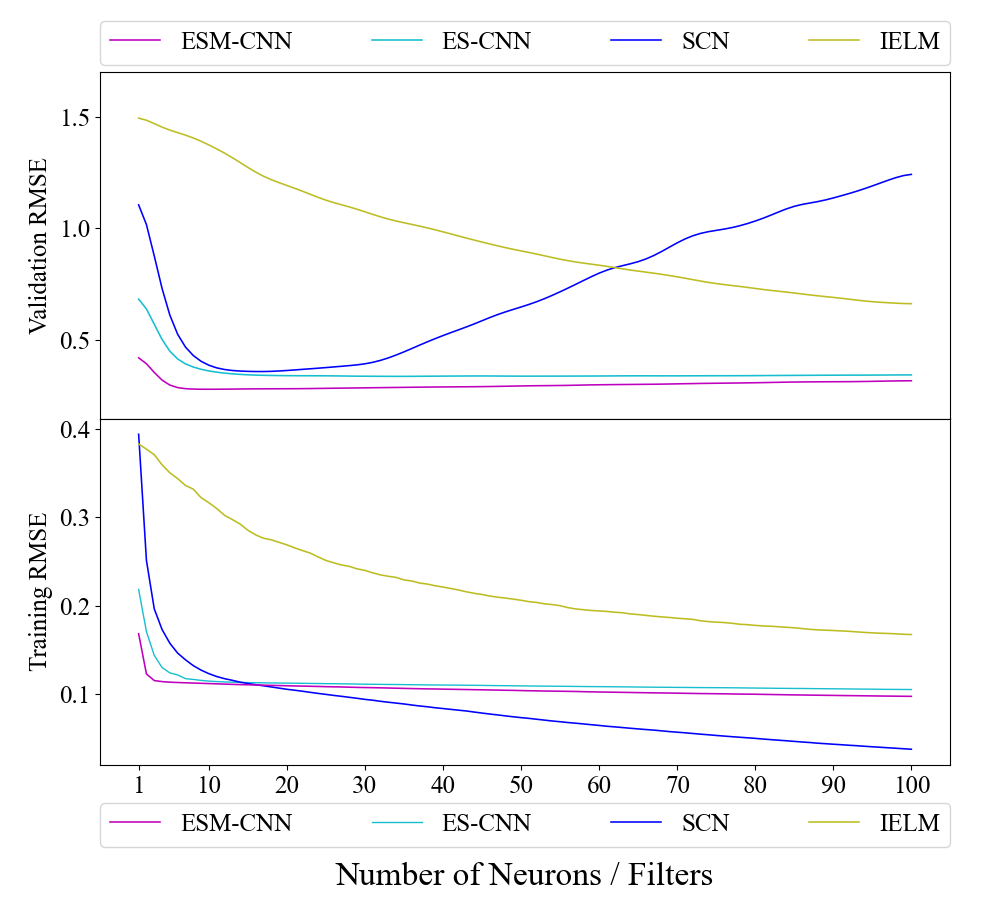
\includegraphics[width = 0.95\textwidth]{float/ch.cnn/sili_H1_revise.png}
            \subcaption{ ILI, $H = 1$ }
        \end{minipage}
        \begin{minipage}[b]{0.32\textwidth}
            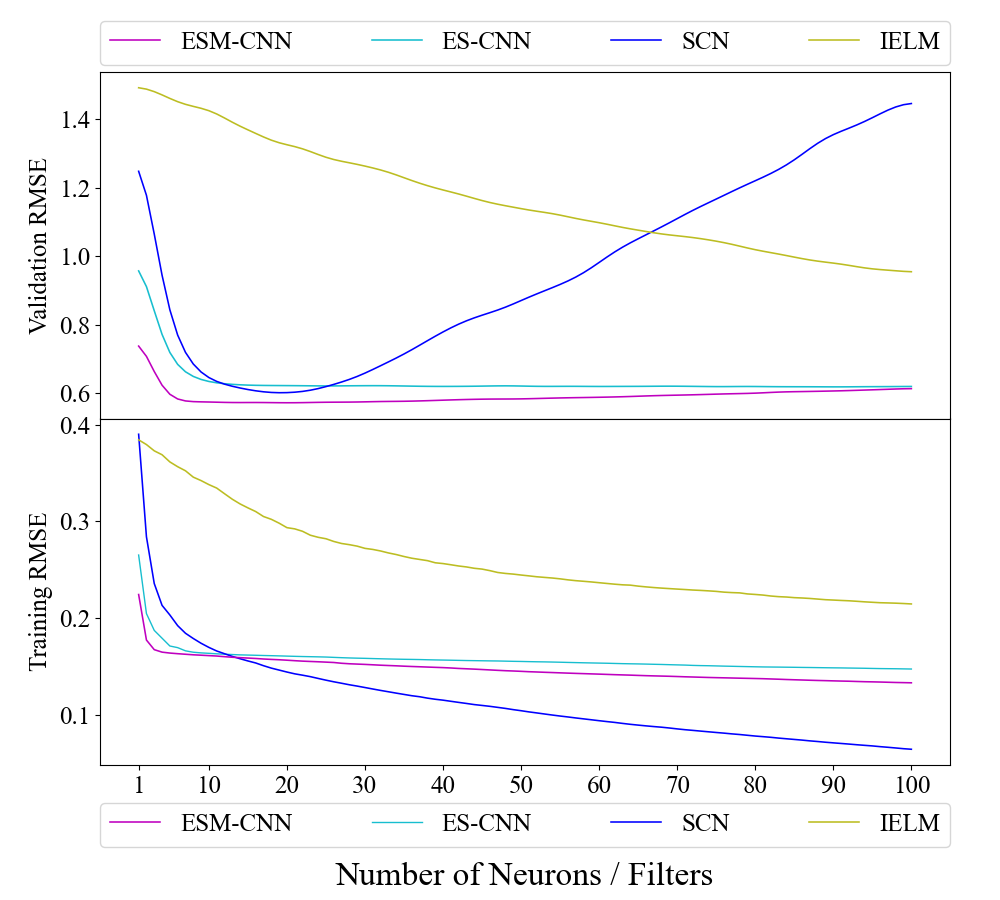
\includegraphics[width = 0.95\textwidth]{float/ch.cnn/sili_H4_revise.png}
            \subcaption{ ILI, $H = 4$ }
        \end{minipage}
        \begin{minipage}[b]{0.32\textwidth}
            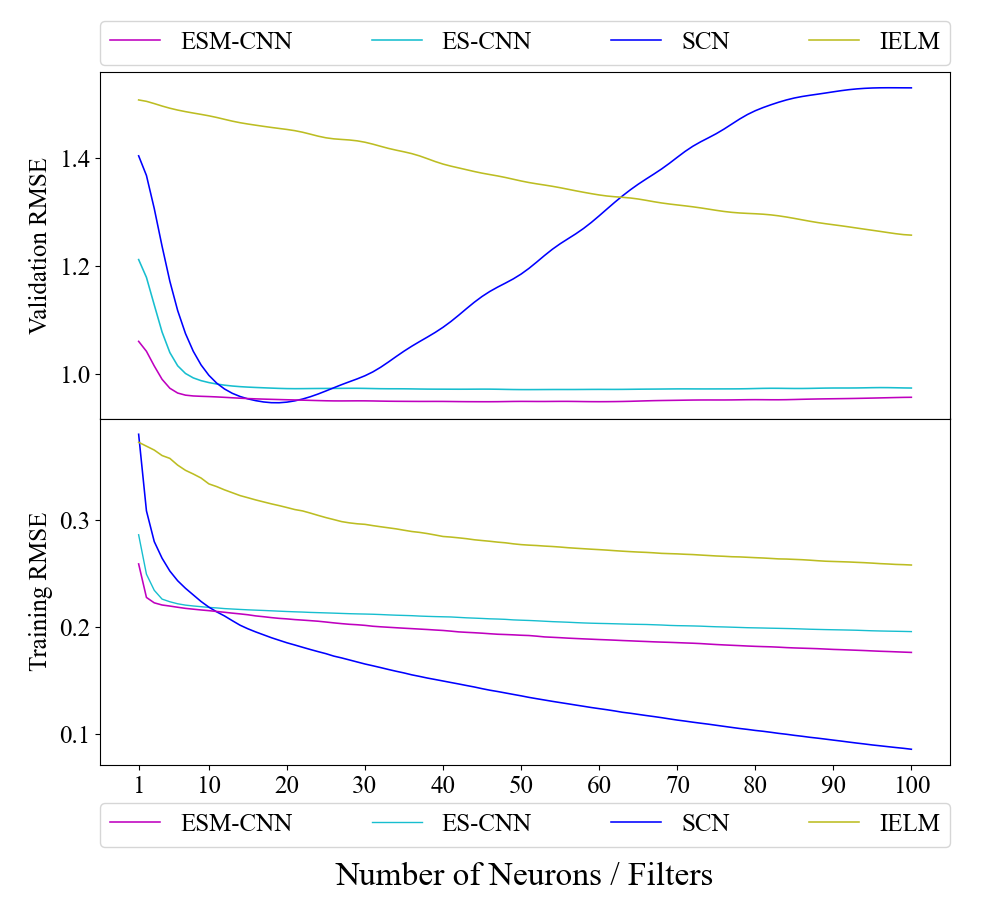
\includegraphics[width = 0.95\textwidth]{float/ch.cnn/sili_H8_revise.png}
            \subcaption{ ILI, $H = 8$ }
        \end{minipage}

        \caption*{ILI数据集上递归增长随机映射神经网络的RMSE曲线}
    \end{figure}
\end{frame}

\begin{frame}
    \frametitle{Conv-SDNN预测模型——收敛性分析}

    \begin{enumerate}
        \item[1)] 同一预测模型在不同预测时长任务上的收敛情况是一致的。
        \item[2)] 尽管SCN模型在不同预测任务的训练集RMSE上都能做出最快收敛,但SCN模型在进行真实预测建模中出现了明显的过拟合现象,而采用误差反馈策略的IELM模型并没有出现过拟合,但表现出最慢的收敛速度。这一对比结果证明了误差反馈策略解决过拟合问题的有效性,同时也指出了误差反馈策略下MLP结构的性能局限性。
        \item[3)] 基于卷积结构的ESM-CNN和ES-CNN在所有的验证集RMSE中都表现出比IELM和SCN更快且更低的收敛效果,证明了基于误差反馈随机映射构造CNN预测模型的收敛性与鲁棒性。
        \item[4)] 与ES-CNN相比,ESM-CNN具备更低的训练集RMSE曲线和测试集RMSE曲线,从收敛性角度再次验证了所提卷积核选择方法的有效性与必要性。
        \item[5)] 在ESM-CNN与ES-CNN的收敛过程中,预测性能的最大增益明显来自于构造过程的前10步,表现出ESM-CNN具备通过牺牲微小性能换来巨大效率提升的平衡策略,从而使得ESM-CNN具有更加广泛和高效的现实应用性。
    \end{enumerate}

\end{frame}

\begin{frame}
    \frametitle{Conv-SDNN预测模型——建模效率分析}
    \begin{table*}[!t]
    \centering
    \footnotesize
    \caption{神经网络模型在AR1、BTC和ILI数据集上的单次平均建模时间(s) \label{tab:time}}
    \resizebox{\textwidth}{!}{\begin{tabular}{ccrrrrrrrrr}
        \toprule
        \multirow{2}{*}{建模方法}   & \multirow{2}{*}{模型} & \multicolumn{3}{c}{AR1} & \multicolumn{3}{c}{BTC} & \multicolumn{3}{c}{ILI}                                           \\\cmidrule(lr){3-5} \cmidrule(lr){6-8}\cmidrule(lr){9-11}
                          &                         & \multicolumn{1}{c}{1} & \multicolumn{1}{c}{3} & \multicolumn{1}{c}{6} & \multicolumn{1}{c}{1} & \multicolumn{1}{c}{3} & \multicolumn{1}{c}{6} & \multicolumn{1}{c}{1} & \multicolumn{1}{c}{4} & \multicolumn{1}{c}{8} \\ \midrule        
        
\multirow{3}{*}{梯度下降} & GS-CNN                  & 74.65                 & 76.95                 & 78.55                 & 93.70                 & 96.45                 & 99.40                 & 67.05                 & 70.25                 & 73.00                 \\
                          & DeepAR                  & 225.25                & 238.95                & 257.70                & 223.75                & 251.10                & 268.65                & 256.80                & 279.10                & 275.30                \\
                          & CLSTM                   & 150.45                & 154.80                & 160.25                & 143.00                & 141.50                & 142.25                & 167.40                & 170.80                & 175.30                \\
\specialrule{0em}{1.5pt}{1.5pt}                          
\multirow{3}{*}{随机映射}   & RVFL                    & \multicolumn{1}{c}{-} & \multicolumn{1}{c}{-} & \multicolumn{1}{c}{-} & \multicolumn{1}{c}{-}  & \multicolumn{1}{c}{-}  & \multicolumn{1}{c}{-}  & \multicolumn{1}{c}{-} & \multicolumn{1}{c}{-} & \multicolumn{1}{c}{-} \\
                          & IELM                    & 2.65                  & 2.85                  & 2.80                  & 3.40                  & 3.30                  & 3.20                  & 2.55                  & 2.55                  & 2.40                  \\
                          & SCN                     & 22.85                 & 57.40                 & 107.75                & 21.10                 & 58.00                 & 111.40                & 16.10                 & 49.60                 & 90.95                 \\
\specialrule{0em}{1.5pt}{1.5pt}                          
\multirow{2}{*}{消融方法} & Stoc-CNN                & \multicolumn{1}{c}{-} & \multicolumn{1}{c}{-} & \multicolumn{1}{c}{-} & \multicolumn{1}{c}{-}  & \multicolumn{1}{c}{-}  & \multicolumn{1}{c}{-}  & \multicolumn{1}{c}{-} & \multicolumn{1}{c}{-} & \multicolumn{1}{c}{-} \\
                          & ES-CNN                  & 6.50                  & 6.40                  & 6.50                  & 6.35                  & 6.50                  & 6.45                  & 6.45                  & 6.50                  & 6.50                  \\
\specialrule{0em}{1.5pt}{1.5pt}                          
所提方法                       & ESM-CNN                 & 9.65                  & 9.65                  & 9.70                  & 7.10                  & 7.25                  & 7.25                  & 7.15                  & 7.15                  & 7.20                  \\ \bottomrule
    \end{tabular}}
\end{table*}

\end{frame}

\begin{frame}
    \frametitle{Conv-SDNN预测模型——小结}

    \textbf{(1)基于卷积结构的SDNN预测模型构造与优化方法}
    \begin{itemize}
        \item 通过代数推导证明了基于该方法所构造的预测模型具有随着卷积核的增加而单调下降的预测误差,以此保证了所提方法的收敛性,且其确定的输出权重与既有方法相比具有更小的$L_2$范数,以此提升了模型的预测稳定性;
        \item 区别于既有方法仅能用相同宽度的卷积核构造单卷积层,通过贪心选择由不同卷积核宽度组成的备选集,使得模型能够在迭代构造模型的过程中自适应确定卷积参数,其构造的单卷积层具备不同宽度的卷积核,使模型借助单卷积层具备不同尺度局部特征的学习能力;
        \item 在人工合成数据、流感阳率数据、原油价格数据和金融指数数据上的实验表明,与梯度下降训练的深度神经网络预测模型相比,基于本方法所构造的模型在具备相近甚至更优的预测准确度同时具备极高的建模效率,验证了所提方法的有效性。
    \end{itemize}

\end{frame}
% \input{body/esn.tex}
% \input{body/dfs.tex}
% \input{body/eto.tex}
% \section{code}

\begin{frame}
    \frametitle{预测建模框架——OpenForecasting}


    \begin{figure}
        \begin{minipage}[t]{0.58\textwidth}
            OpenForecasting:
            \begin{itemize}
                \item 整合既有优秀神经网络建模框架与参数优化框架,提供预测建模通用框架平台
                \item 完备包含时间序列预测建模的数据初始化、数据预处理、模型构造、模型优化和模型评价等构造与评价流程,集成多类别、多结构的现有对比预测方法
            \end{itemize}

            \vspace{1em}
            已开源:
            
            https://github.com/Analytics-for-Forecasting/
            
            OpenForecasting.
        \end{minipage}
        \hfill
        \begin{minipage}[t]{0.4\textwidth}
            框架需求:
    \begin{itemize}
        \item 数据管理功能:
        \begin{itemize}
            \item 异构数据结构化方法
            \item 输入数据预处理方法
            \item 输出数据评价方法
        \end{itemize}
    \end{itemize}

    \begin{itemize}
        \item 模型构造功能:
        \begin{itemize}
            \item 单元化、模块化、标准化
            \item 多类别、多结构
        \end{itemize}
    \end{itemize}
    
    \begin{itemize}
        \item 模型优化功能:
        \begin{itemize}
            \item 多种超参数优化方法
            \item 多种权重参数优化方法
        \end{itemize}
    \end{itemize}
        \end{minipage}
    \end{figure}

\end{frame}

\begin{frame}
    \frametitle{预测建模框架——OpenForecasting}
    \centering
    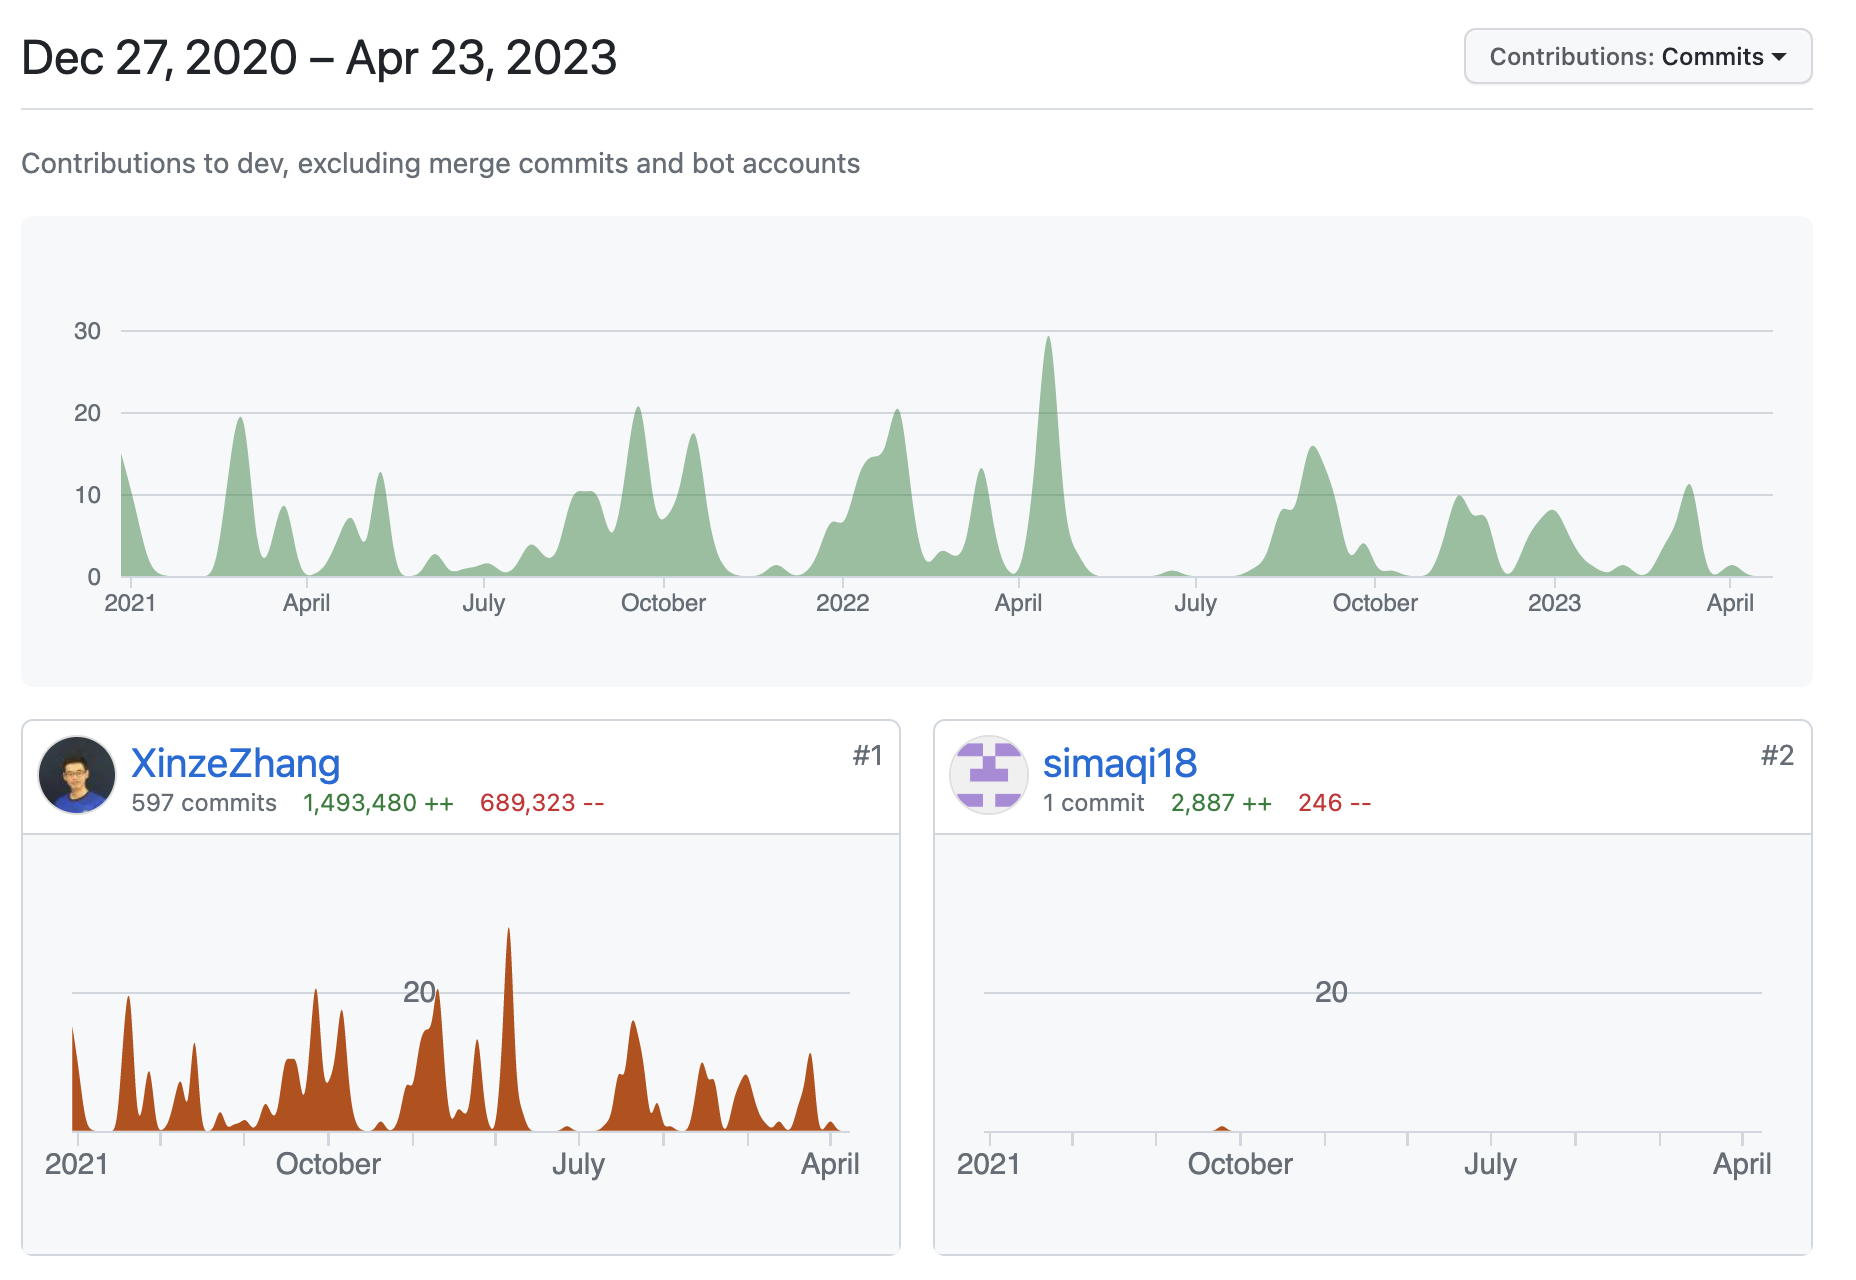
\includegraphics[width = 0.83\linewidth]{float/ch.univ/code2.png}

\end{frame} 
\section{last}

\begin{frame}
    \frametitle{总结与展望}
    % 主要工作:

    % \begin{itemize}
    %     \item 特定结构构造与优化方法研究
    %     \begin{itemize}
    %         \item 基于卷积结构的SDNN预测模型构造与优化方法
    %         \item 基于循环结构的SDNN预测模型构造与优化方法
    %     \end{itemize}
    %     \item 一般结构优化方法研究
    %   \begin{itemize}
    %         \item SDNN预测模型的二重特征结构选择方法
    %     \end{itemize}
    %     \item 混合结构优化方法研究
    %     \begin{itemize}
    %         \item SDNN预测模型的混合结构生长与优化方法
    %     \end{itemize}
    % \end{itemize}
    \begin{figure}[!t]
        \begin{minipage}{0.45\textwidth}
            \centering
            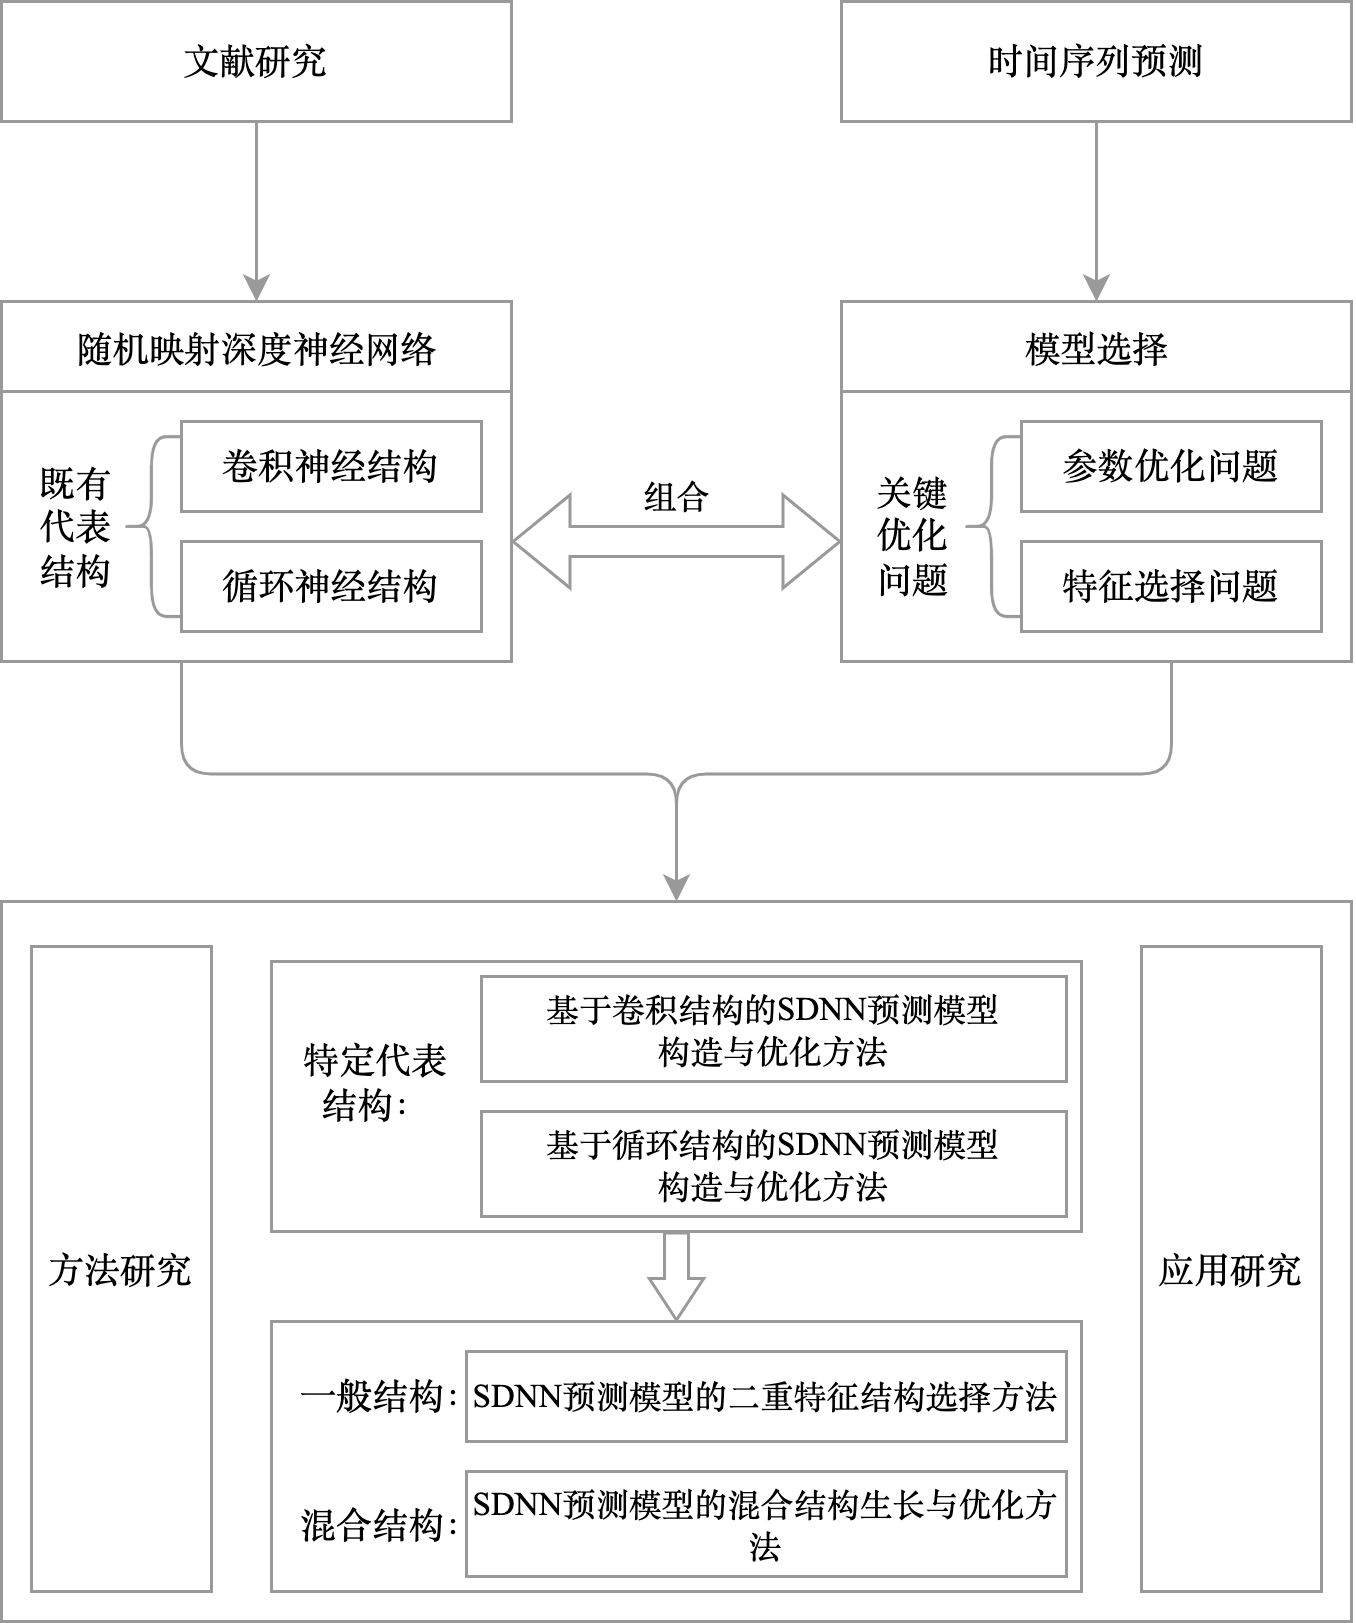
\includegraphics[width=0.825\linewidth]{float/ch.intro/thesis_arch.png}
            \caption*{本研究技术路线}
        \end{minipage}
        \hfill
        \begin{minipage}{0.45\textwidth}
            \centering
            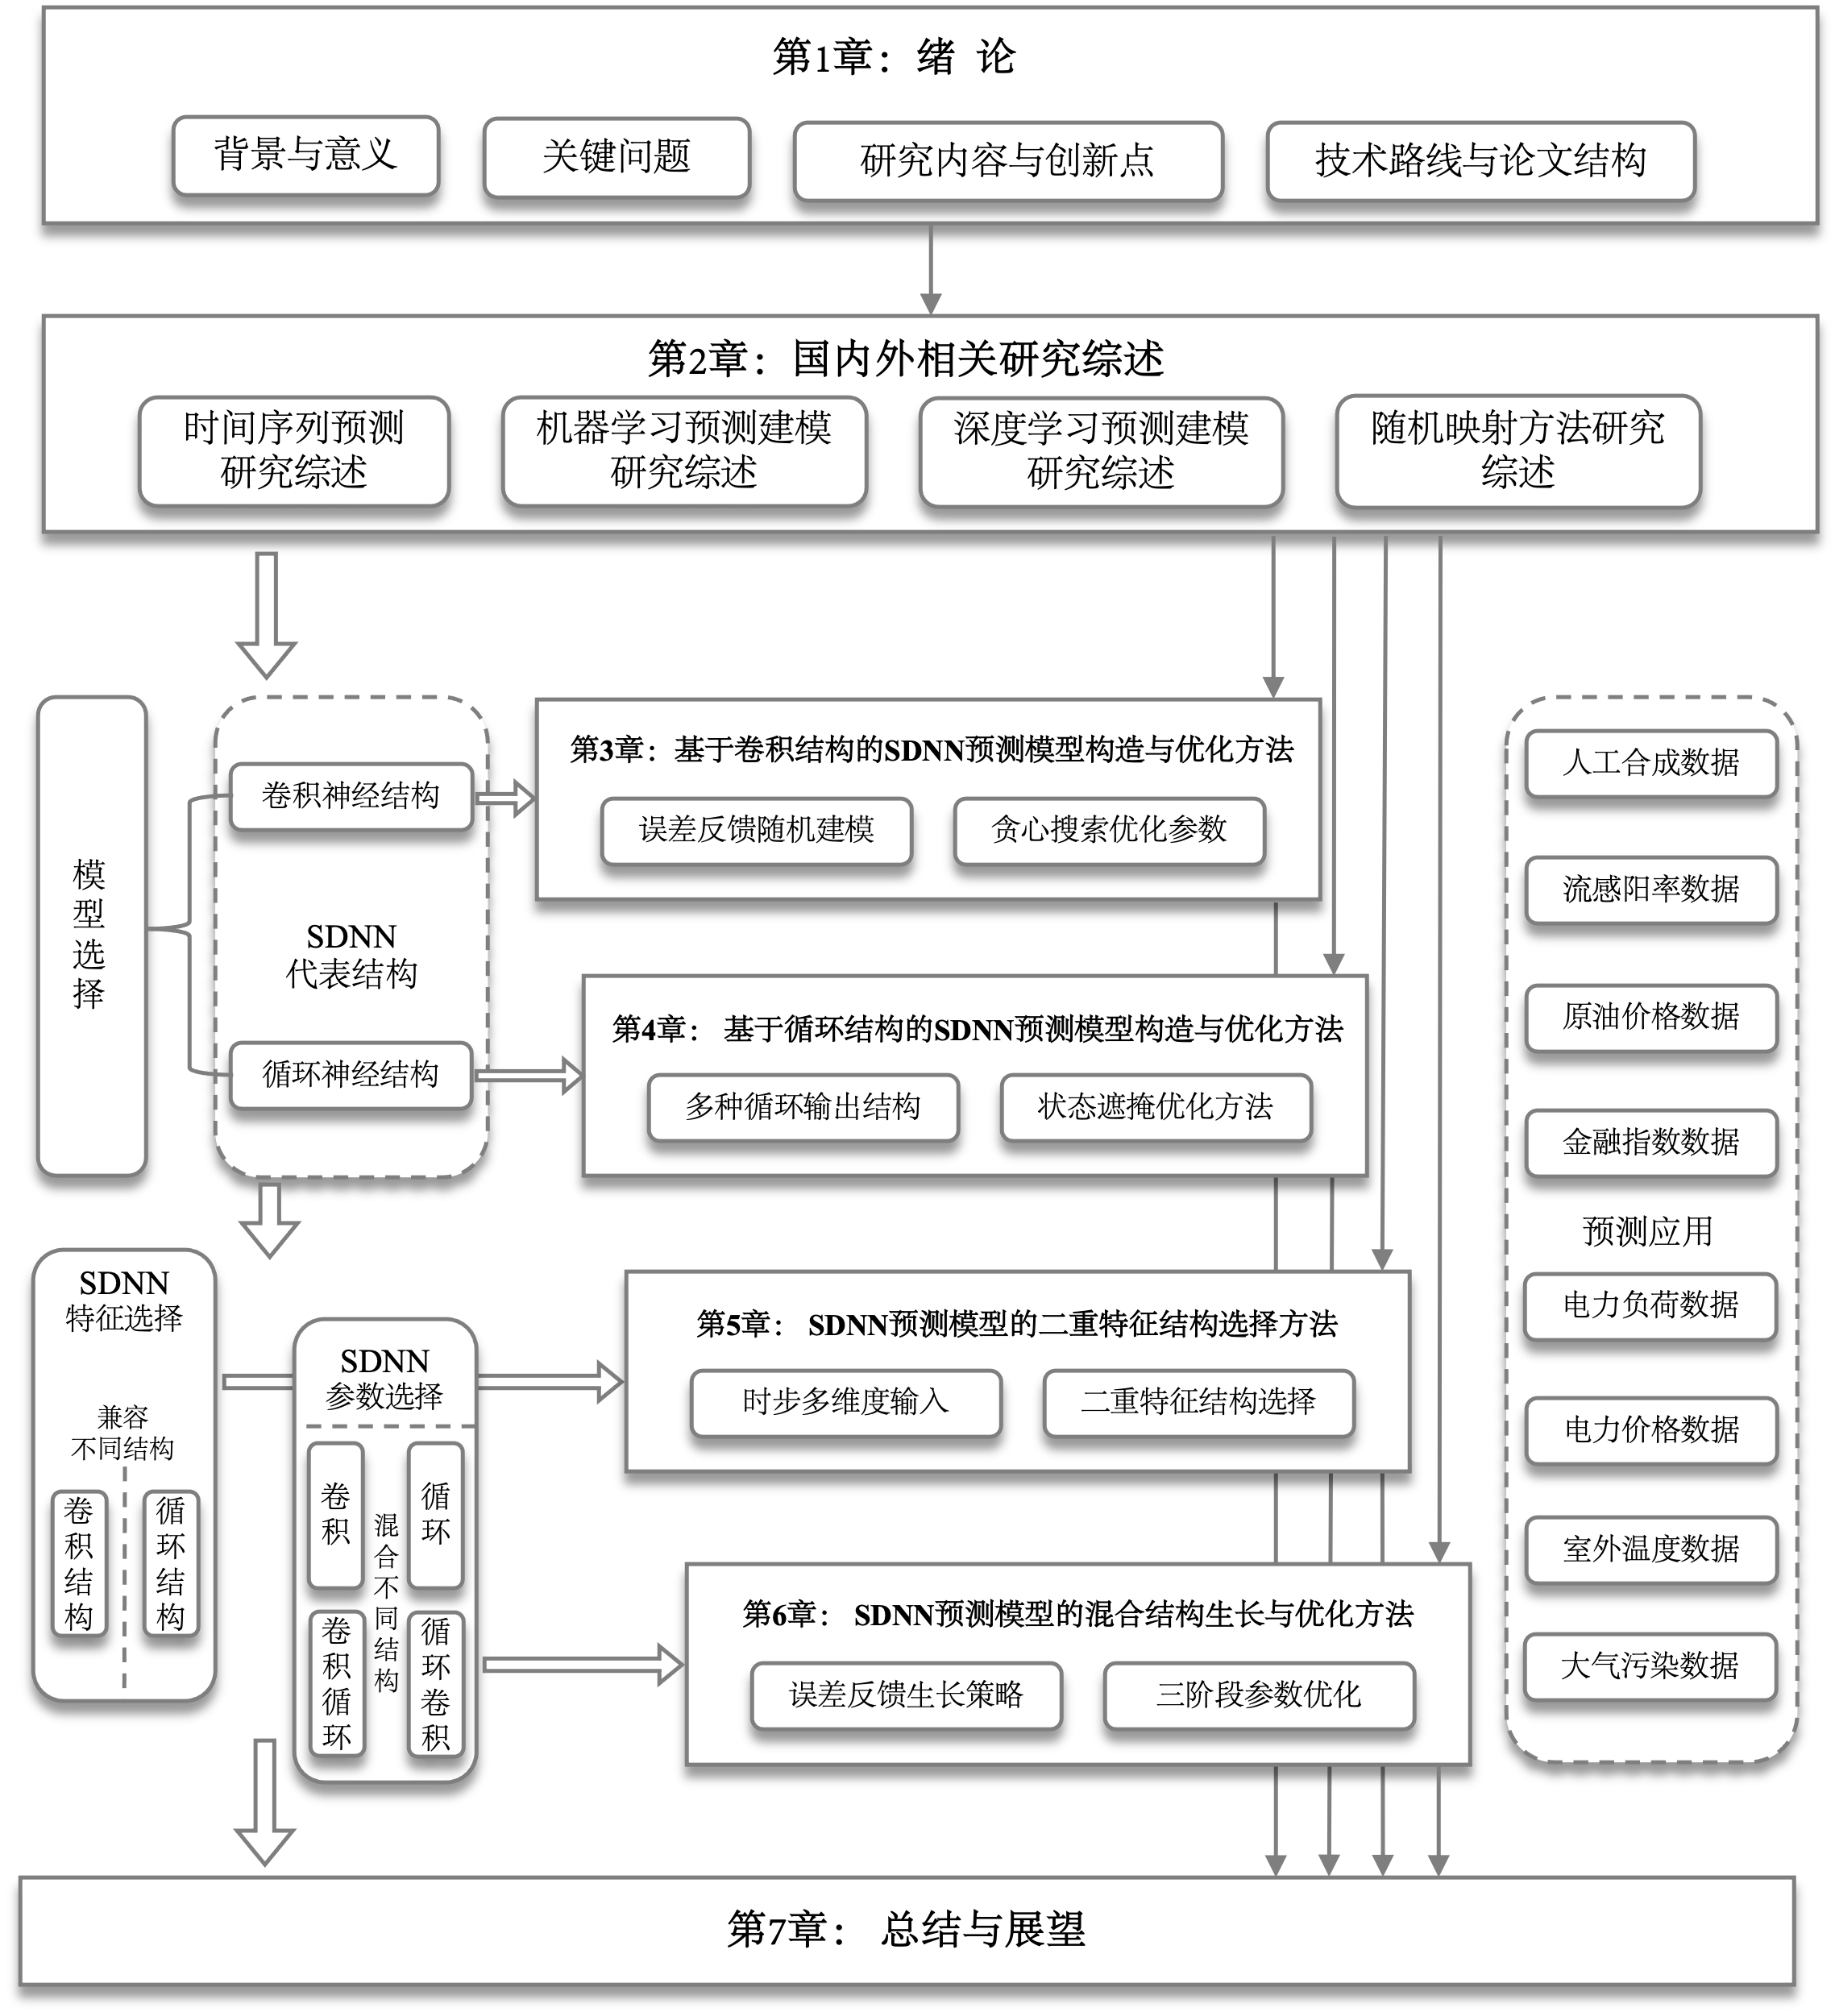
\includegraphics[width=0.9\linewidth]{float/ch.intro/thesis_content.png}
            \caption*{本论文主要结构}
        \end{minipage}

    \end{figure}
\end{frame}

\begin{frame}
    \frametitle{研究展望}
         
    卷积结构的SDNN预测模型构造与优化方法:
    \begin{itemize}
        \item 可以通过计算不同方法的时间复杂度与空间复杂度,从而精确比较各方法的建模效率优劣
        \item 基于历史数据训练和构造的模型不一定适应于时变的时间序列数据,因此可以通过考虑剪枝策略,设计模型结构对时变时间序列数据的自适应方法
    \end{itemize}

    循环结构的SDNN预测模型构造与优化方法研究
    \begin{itemize}
        \item 未有考虑状态遮掩机制对于不同随机循环隐藏结构的影响,因此可以进行状态遮掩输出结构在其他随机循环隐藏结构(如GESN或DESN结构)上的迁移实验
        \item 在梯度下降的RNN预测模型训练中同样存在类似的问题,因此可以通过设计基于状态遮掩的新颖梯度下降损失函数,提升RNN预测模型的预测效果。
    \end{itemize}

\end{frame}

\begin{frame}
    \frametitle{研究展望}
         
    SDNN预测模型的二重特征结构选择方法研究:
    \begin{itemize}
        \item 二维的时间序列输入特征结构同样适用于梯度下降训练的CNN与RNN模型,因此可以考虑进行二重特征结构选择方法在训练的深度神经网络模型上的迁移实验
        \item 可以考虑联立循环结构SDNN预测模型的输入特征时步掩码和隐藏特征时步掩码,构建多阶段整体优化的循环结构SDNN预测模型,进一步提升其预测效果
    \end{itemize}

    SDNN预测模型的混合结构生长与优化方法研究
    \begin{itemize}
        \item 限定于SDNN预测模型的输入与隐藏结构,未有考虑输出结构的生长与优化问题,因此可以构造混合多种不同输出结构的自适应端到端预测模型
        \item 随机映射方法下的误差反馈生长策略并不适用于梯度下降方法,因此可以设计基于误差反馈的子网络新颖权重训练方法,构造具有收敛保证的混合结构DNN预测模型
    \end{itemize}

\end{frame}




\begin{frame}
    \frametitle{总结与展望}

    围绕上述不足之处与改进方法,未来的研究工作将持续探索时间序列预测建模技术的更多可能与思路。
    
    希望借助随机映射方法,通过进一步的学习与交流,完善深度学习预测模型的解释性研究,探寻预测模型与其优化方法在构造选择效率与预测性能提升间的更佳平衡,使其在更为广泛的应用领域发挥可信且有效的支撑作用。


    \vspace*{1em}
    \(\circ\)衷心感谢博士生导师鲍玉昆教授、计算机科技与技术学院的何琨教授、硕士研究生导师蔡淑琴教授对我的指导。

    \(\circ\)感谢预答辩委员会的胡斌教授、王林教授、杨彦武教授和吴庆华教授。
    
    \(\circ\)感谢我的爱人、父母、朋友、师弟师妹,以及所有的支持者!

\end{frame}
    

% \input{1.inro.tex}
% \input{2.cnn.tex}
% \input{3.esn.tex}
% \input{5.dfs.tex}
% \input{4.eto.tex}
% % \input{6.univ.tex}
% \input{7.last.tex}
% \begin{frame}
%   \frametitle{谢谢各位评委老师!}
%   \centering
%   \includegraphics[width=1\textwidth]{fig/aboutme.png}

% \end{frame}

\end{document}